\documentclass{article}

\newcommand{\accuracyTable}{{
\begin{table*}[t]
\centering
\captionof{table}{Performance of LLaMA-7B compressed by \sysname, \sysname \texttt{(W)}, and baselines under different compression ratio (corresponding weight memory is listed inside bracket) on two language modeling datasets (measured by perplexity  (\textcolor{mygreen}{$\downarrow$})), eight common sense reasoning datasets (six measured by both individual and average accuracy (\textcolor{mygreen}{$\uparrow$}), TruthfulQA measured by BLEU score (\textcolor{mygreen}{$\uparrow$}), and GSM8K measured by Exact Match Accuracy (\textcolor{mygreen}{$\uparrow$})). The best performance is marked in bold. The relative performance gain compared to the best-performing baseline is marked in green inside bracket.
}
\vspace{-2mm}
\resizebox{1\textwidth}{!}{%}
\begin{tabular}{ccccccccccccc}
\midrule
\multicolumn{1}{c|}{\textsc{Ratio (Mem.)}}       & \multicolumn{1}{c|}{\textsc{Method}}    & WikiText-2\textcolor{mygreen}{$\downarrow$} & \multicolumn{1}{c|}{C4\textcolor{mygreen}{$\downarrow$}} & Openb. & ARC\_e & WinoG. & HellaS.  & PIQA & MathQA & \textbf{Average\textcolor{mygreen}{$\uparrow$}}  & TruthfulQA\textcolor{mygreen}{$\uparrow$} & GSM8K\textcolor{mygreen}{$\uparrow$}      \\ \midrule
\multicolumn{1}{c|}{\color[HTML]{9B9B9B}0\% (13.5 GB)}  & \multicolumn{1}{c|}{\color[HTML]{9B9B9B}Original}  & {\color[HTML]{9B9B9B}5.68}     & \multicolumn{1}{c|}{\color[HTML]{9B9B9B}7.34}      & {\color[HTML]{9B9B9B} 0.34} & {\color[HTML]{9B9B9B} 0.75} & {\color[HTML]{9B9B9B} 0.70} & {\color[HTML]{9B9B9B} 0.57} & {\color[HTML]{9B9B9B} 0.79} & {\color[HTML]{9B9B9B} 0.27} & {\color[HTML]{9B9B9B} 0.57}    & {\color[HTML]{9B9B9B}0.30}  & {\color[HTML]{9B9B9B}0.09}\\ \midrule
\multicolumn{1}{c|}{\multirow{4}{*}{20\% (10.2 GB)}} & \multicolumn{1}{c|}{SVD}      & 20061                     & \multicolumn{1}{c|}{18800}          & 0.05  & 0.04  & 0.01  & 0.03  & 0.02  & 0.03  & 0.03  & 0.00   & 0.00 \\
\multicolumn{1}{c|}{}                     & \multicolumn{1}{c|}{FWSVD}     & 1727                     & \multicolumn{1}{c|}{1511}                      & 0.09  & 0.11  & 0.05  & 0.08  & 0.10  & 0.05  & 0.08  & 0.00   & 0.00 \\
\multicolumn{1}{c|}{}                     & \multicolumn{1}{c|}{ASVD}      & 11.14                   & \multicolumn{1}{c|}{15.93}                      & 0.29  & 0.53  & 0.64  & 0.41  & 0.68  & 0.17  & 0.45  & 0.21   & 0.04\\ \cmidrule{2-13} 
\multicolumn{1}{c|}{}                     & \multicolumn{1}{c|}{\xin{\sysname \texttt{(W)}}}  & 7.94 (\textcolor{mygreen}{$\downarrow$29\%})  & \multicolumn{1}{c|}{15.84 (\textcolor{mygreen}{$\downarrow$1\%})}       & 0.31  & 0.62  & 0.61 & 0.45  & 0.71  & 0.21  & 0.49 (\textcolor{mygreen}{$\uparrow$9\%})  & 0.26 (\textcolor{mygreen}{+0.05})  & 0.05 (\textcolor{mygreen}{+0.01})\\ 
\multicolumn{1}{c|}{}                     & \multicolumn{1}{c|}{\sysname}  & \textbf{7.73} (\textcolor{mygreen}{$\downarrow$31\%})  & \multicolumn{1}{c|}{\textbf{12.23} (\textcolor{mygreen}{$\downarrow$23\%})}       & \textbf{0.33}  & \textbf{0.67}  & \textbf{0.69 } & \textbf{0.55}  & \textbf{0.79}  & \textbf{0.26}  & \textbf{0.55} (\textcolor{mygreen}{$\uparrow$22\%})  & \textbf{0.28} (\textcolor{mygreen}{+0.07})  & \textbf{0.08} (\textcolor{mygreen}{+0.04})\\ \midrule

\multicolumn{1}{c|}{\multirow{4}{*}{40\% (7.76 GB)}} & \multicolumn{1}{c|}{SVD}      & 52489                    & \multicolumn{1}{c|}{47774}           & 0.04  & 0.04  & 0.05  & 0.01  & 0.03  & 0.02  & 0.03  & 0.00   & 0.00\\
\multicolumn{1}{c|}{}                     & \multicolumn{1}{c|}{FWSVD}     & 18156                     & \multicolumn{1}{c|}{12847}                    & 0.06  & 0.05  & 0.02  & 0.00  & 0.05  & 0.03  & 0.04  & 0.00   & 0.00\\
\multicolumn{1}{c|}{}                     & \multicolumn{1}{c|}{ASVD}      & 1407                 & \multicolumn{1}{c|}{1109}                          & 0.08  & 0.11  & 0.09  & 0.08  & 0.13  & 0.08  & 0.10  & 0.01   & 0.00\\ \cmidrule{2-13} 
\multicolumn{1}{c|}{}                     & \multicolumn{1}{c|}{\xin{\sysname \texttt{(W)}}}  & 13.73 (\textcolor{mygreen}{$\downarrow$99\%}) & \multicolumn{1}{c|}{75.42 (\textcolor{mygreen}{$\downarrow$93\%})}        & 0.25  & 0.33  & 0.55  & 0.40  & 0.63  & 0.12  & 0.38 (\textcolor{mygreen}{$\uparrow$280\%})  & 0.17 (\textcolor{mygreen}{+0.17})   & 0.02 (\textcolor{mygreen}{+0.02})\\ 
\multicolumn{1}{c|}{}                     & \multicolumn{1}{c|}{\sysname}  & \textbf{9.27} (\textcolor{mygreen}{$\downarrow$99\%}) & \multicolumn{1}{c|}{\textbf{15.63} (\textcolor{mygreen}{$\downarrow$99\%})}        & \textbf{0.29}  & \textbf{0.59}  & \textbf{0.68}  & \textbf{0.52}  & \textbf{0.69}  & \textbf{0.20}  & \textbf{0.50} (\textcolor{mygreen}{$\uparrow$400\%})  & \textbf{0.24} (\textcolor{mygreen}{+0.23})   & \textbf{0.07} (\textcolor{mygreen}{+0.07})\\ \midrule
\multicolumn{1}{c|}{\multirow{4}{*}{60\% (5.35 GB)}} & \multicolumn{1}{c|}{SVD}      & 105474                     & \multicolumn{1}{c|}{106976}        & 0.01  & 0.03  & 0.01  & 0.00  & 0.01  & 0.02  & 0.01  & 0.00   & 0.00\\
\multicolumn{1}{c|}{}                     & \multicolumn{1}{c|}{FWSVD}     & 32194                     & \multicolumn{1}{c|}{29292}                    & 0.06  & 0.02  & 0.01  & 0.01  & 0.02  & 0.03  & 0.03  & 0.00   & 0.00\\
\multicolumn{1}{c|}{}                     & \multicolumn{1}{c|}{ASVD}      & 57057                  & \multicolumn{1}{c|}{43036}                       & 0.05  & 0.04  & 0.06  & 0.09  & 0.08  & 0.05  & 0.06  & 0.00   & 0.00\\ \cmidrule{2-13} 
\multicolumn{1}{c|}{}                     & \multicolumn{1}{c|}{\xin{\sysname \texttt{(W)}}}  & 66.62 (\textcolor{mygreen}{$\downarrow$99\%}) & \multicolumn{1}{c|}{471.83 (\textcolor{mygreen}{$\downarrow$99\%})}       & 0.10  & 0.05  & 0.17  & 0.10  & 0.21  & 0.04  & 0.11 (\textcolor{mygreen}{$\uparrow$83\%})  & 0.01 (\textcolor{mygreen}{+0.01})   & 0.00 (\textcolor{mygreen}{+0.00})\\ 
\multicolumn{1}{c|}{}                     & \multicolumn{1}{c|}{\sysname}  & \textbf{15.00} (\textcolor{mygreen}{$\downarrow$99\%}) & \multicolumn{1}{c|}{\textbf{26.26} (\textcolor{mygreen}{$\downarrow$99\%})}       & \textbf{0.18}  & \textbf{0.42}  & \textbf{0.44}  & \textbf{0.31}  & \textbf{0.35}  & \textbf{0.12}  & \textbf{0.30} (\textcolor{mygreen}{$\uparrow$400\%})  & \textbf{0.14} (\textcolor{mygreen}{+0.14})   & \textbf{0.04} (\textcolor{mygreen}{+0.04})\\ \midrule
\multicolumn{1}{c|}{\multirow{4}{*}{80\% (2.58 GB)}} & \multicolumn{1}{c|}{SVD}      & 687291                     & \multicolumn{1}{c|}{708243}        & 0.00  & 0.01  & 0.02  & 0.01  & 0.01  & 0.00  & 0.01  & 0.00   & 0.00\\
\multicolumn{1}{c|}{}                     & \multicolumn{1}{c|}{FWSVD}     & 96872                    & \multicolumn{1}{c|}{89243}                     & 0.01  & 0.02  & 0.00  & 0.01  & 0.01  & 0.00  & 0.01  & 0.00   & 0.00\\
\multicolumn{1}{c|}{}                     & \multicolumn{1}{c|}{ASVD}      & 80425                 & \multicolumn{1}{c|}{67927}                        & 0.04  & 0.03  & 0.03  & 0.02  & 0.01  & 0.01  & 0.03  & 0.00   & 0.00\\ \cmidrule{2-13} 
\multicolumn{1}{c|}{}                     & \multicolumn{1}{c|}{\xin{\sysname \texttt{(W)}}}  & 1349 (\textcolor{mygreen}{$\downarrow$98\%}) & \multicolumn{1}{c|}{6224 (\textcolor{mygreen}{$\downarrow$91\%})}       & 0.07  & 0.03  & 0.04  & 0.02  & 0.07  & 0.01  & 0.04 (\textcolor{mygreen}{$\uparrow$33\%})  & 0.00 (\textcolor{mygreen}{+0.00})  & 0.00 (\textcolor{mygreen}{+0.00})\\ 
\multicolumn{1}{c|}{}                     & \multicolumn{1}{c|}{\sysname}  & \textbf{31.79} (\textcolor{mygreen}{$\downarrow$99\%}) & \multicolumn{1}{c|}{\textbf{43.71} (\textcolor{mygreen}{$\downarrow$99\%})}       & \textbf{0.11}  & \textbf{0.23}  & \textbf{0.21}  & \textbf{0.14}  & \textbf{0.17}  & \textbf{0.08}  & \textbf{0.16} (\textcolor{mygreen}{$\uparrow$433\%})  & \textbf{0.04} (\textcolor{mygreen}{+0.04})  & \textbf{0.02} (\textcolor{mygreen}{+0.02})\\ \midrule
\end{tabular}
}
\vspace{-4mm}
\label{tab:dataset_acc}
\end{table*}
}}
%%%%%%%%%%%%%%%%%%%%%%%%%%%%%%%%%%%%%%%%%%%%%%%%%%%

\newcommand{\differntllmaccuracyTable}{{
\begin{table}[t]
\centering
\captionof{table}{Perplexity ($\downarrow$) of \sysname, \sysname \texttt{(W)}, and baselines on WikiText-2 and the average accuracy ($\uparrow$) of the six common sense reasoning datasets of four different LLMs -- OPT-6.7B, LLaMA 2-7B, Mistral-7B, and Vicuna-7B -- under 20\% compression ratio. The relative performance gain compared to the best-performing baseline is marked in green color inside bracket.}
\vspace{-2mm}
\resizebox{1\textwidth}{!}{%
\begin{tabular}{c|cc|cc|cc|cc}
% \toprule[0.01pt]
\midrule
& \multicolumn{2}{c}{OPT-6.7B}   & \multicolumn{2}{c}{\textsc{LLaMA 2-7B}}    & \multicolumn{2}{c}{\textsc{Mistral-7B}}        & \multicolumn{2}{c}{\textsc{Vicuna-7B}} \\\midrule
\textsc{Method} & Perplexity\textcolor{mygreen}{$\downarrow$}    & Accuracy\textcolor{mygreen}{$\uparrow$}    & Perplexity\textcolor{mygreen}{$\downarrow$}    & Accuracy\textcolor{mygreen}{$\uparrow$}  & Perplexity\textcolor{mygreen}{$\downarrow$}    & Accuracy\textcolor{mygreen}{$\uparrow$}  & Perplexity\textcolor{mygreen}{$\downarrow$}    & Accuracy\textcolor{mygreen}{$\uparrow$} \\ \midrule
\color[HTML]{9B9B9B}Original       & \color[HTML]{9B9B9B}10.86          & \color[HTML]{9B9B9B}0.52         & \color[HTML]{9B9B9B}5.47            & \color[HTML]{9B9B9B}0.57      & \color[HTML]{9B9B9B}5.25          & \color[HTML]{9B9B9B}0.61         & \color[HTML]{9B9B9B}6.78            & \color[HTML]{9B9B9B}0.56    \\\midrule
SVD       & 66275      & 0.03         & 18192             & 0.09      & 159627        & 0.03         & 18644            & 0.05    \\
FWSVD     & 14559      & 0.06         & 2360              & 0.12      & 6357         & 0.08          & 2758              & 0.09 \\
ASVD      & 82.00      & 0.32         & 10.10             & 0.36      & 13.72         & 0.32         & 16.23             & 0.33     \\ \midrule
\xin{\sysname \texttt{(W)}}  & 16.04 (\textcolor{mygreen}{$\downarrow$80\%})         & 0.41 (\textcolor{mygreen}{$\uparrow$28\%})           &  8.50 (\textcolor{mygreen}{$\downarrow$16\%})          & 0.53 (\textcolor{mygreen}{$\uparrow$47\%})      & 10.21 (\textcolor{mygreen}{$\downarrow$26\%})         & 0.42 (\textcolor{mygreen}{$\uparrow$24\%})           &  8.41 (\textcolor{mygreen}{$\downarrow$48\%})          & 0.51 (\textcolor{mygreen}{$\uparrow$55\%})   \\
\sysname  & \textbf{14.47} (\textcolor{mygreen}{$\downarrow$82\%})         & \textbf{0.49} (\textcolor{mygreen}{$\uparrow$53\%})           &  \textbf{7.73} (\textcolor{mygreen}{$\downarrow$23\%})          & \textbf{0.54} (\textcolor{mygreen}{$\uparrow$50\%})      & \textbf{7.47} (\textcolor{mygreen}{$\downarrow$45\%})         & \textbf{0.55} (\textcolor{mygreen}{$\uparrow$72\%})           &  \textbf{7.43} (\textcolor{mygreen}{$\downarrow$54\%})          & \textbf{0.54} (\textcolor{mygreen}{$\uparrow$64\%})   \\ \midrule
% \bottomrule[0.01pt]
\end{tabular}
}
\vspace{-4mm}
\label{tab:different_llm_acc}
\end{table}
}}

%%%%%%%%%%%%%%%%%%%%%%%%%%%%%%%%%%%%%%%%%%%%%%%%%%%%%%

\newcommand{\largellmaccuracyTable}{{
\centering
\captionof{table}{Perplexity ($\downarrow$) of \sysname, \sysname \texttt{(W)}, and baselines on WikiText-2 and the average accuracy ($\uparrow$) of the six classification datasets of LLaMA-13B and LLaMA-30B under 20\% compression ratio. The relative performance gain compared to the best-performing baseline is marked in green color inside bracket.}
\vspace{-2mm}
\resizebox{0.48\textwidth}{!}{%
\begin{tabular}{c|cc|cc}
\midrule
& \multicolumn{2}{c}{\textsc{LLaMA-13B}}    & \multicolumn{2}{c}{\textsc{LLaMA-30B}}         \\\midrule
\textsc{Method}     & Perplexity\textcolor{mygreen}{$\downarrow$}    & Accuracy\textcolor{mygreen}{$\uparrow$}       & Perplexity\textcolor{mygreen}{$\downarrow$}    & Accuracy\textcolor{mygreen}{$\uparrow$}    \\ \midrule
\color[HTML]{9B9B9B}Original                 & \color[HTML]{9B9B9B}5.09        & \color[HTML]{9B9B9B}0.59           & \color[HTML]{9B9B9B}4.10         & \color[HTML]{9B9B9B}0.61 \\\midrule
SVD                 & 946.31        & 0.21           & 54.11         & 0.33            \\
FWSVD               & 15.98         & 0.43           & 20.54         & 0.42             \\
ASVD                & 6.74          & 0.54           & 22.71         & 0.44             \\ \midrule
\xin{\sysname \texttt{(W)}}            &  6.61 (\textcolor{mygreen}{$\downarrow$2\%})         & 0.54 (\textcolor{mygreen}{$\uparrow$0\%})       & 5.63 (\textcolor{mygreen}{$\downarrow$73\%})             & 0.57 (\textcolor{mygreen}{$\uparrow$30\%})          \\
\sysname            &  \textbf{6.43} (\textcolor{mygreen}{$\downarrow$5\%})         & \textbf{0.55} (\textcolor{mygreen}{$\uparrow$2\%})       &\textbf{5.14} (\textcolor{mygreen}{$\downarrow$75\%})             & \textbf{0.59} (\textcolor{mygreen}{$\uparrow$34\%})          \\ \midrule
\end{tabular}
}
\vspace{-5mm}
\label{tab:large_llm_acc}
}}

%%%%%%%%%%%%%%%%%%%%%%%%%%%%%%%%%%%%%%%%%%%%

\newcommand{\loraTable}{{
\centering
\captionof{table}{Perplexity of LLaMA-7B compressed by \sysname under 20\% to 80\% compression ratio on WikiText-2 with different updating orders.}
\vspace{1mm}
\resizebox{1\textwidth}{!}{%
\begin{tabular}{c|cccc}
\midrule
\textsc{Updating Order}     & 20\%      & 40\%      & 60\%   & 80\%   \\ \midrule
$W'_u$ first, then $W'_v$         & 7.85     & 9.32        & \textbf{13.20} (\textcolor{mygreen}{$\downarrow$1\%})  & \textbf{31.67}(\textcolor{mygreen}{$\downarrow$1\%}) \\ \midrule
$W'_v$ first, then $W'_u$          & \textbf{7.73} (\textcolor{mygreen}{$\downarrow$2\%})      & \textbf{9.27} (\textcolor{mygreen}{$\downarrow$1\%})         & 15.00    & 31.79  \\ \midrule
\end{tabular}
}
\label{tab:lora_acc}
}}

%%%%%%%%%%%%%%%%%%%%%%%%%%%%%%%%%%%%%%%%%%%%
\newcommand{\sensitivityTable}{{
\centering
\captionof{table}{Perplexity ($\downarrow$) of compressed LLaMA-7B on WikiText-2 under different compression ratios. \sysname \texttt{(W)} denotes the version of \sysname with truncation-aware data whitening only; \sysname \texttt{(U)} denotes the version of \sysname with parameter update with sequential low-rank approximation only; The relative performance gain compared to ASVD is marked in green color inside bracket.}
\vspace{5mm}
\resizebox{1\textwidth}{!}{%
% \tiny
\begin{tabular}{c|c|c|c}
% \toprule[0.01pt]
\midrule
\textsc{Method} & \multicolumn{1}{c}{\textsc{20\%}}  &\multicolumn{1}{c}{\textsc{40\%}}  &\multicolumn{1}{c}{\textsc{60\%}}     \\ \midrule          
ASVD              & 11.14                 & 1407              & 57057                        \\ \midrule
\sysname \texttt{(W)}      & 7.94 (\textcolor{mygreen}{$\downarrow$29\%})            & 13.11 (\textcolor{mygreen}{$\downarrow$99\%})          & 42.30 (\textcolor{mygreen}{$\downarrow$99\%})     \\ \midrule
\sysname \texttt{(U)}      & 10.12 (\textcolor{mygreen}{$\downarrow$9\%})            & 19.28 (\textcolor{mygreen}{$\downarrow$99\%})          & 49.88 (\textcolor{mygreen}{$\downarrow$99\%})     \\ \midrule
\sysname  & \textbf{7.73} (\textcolor{mygreen}{$\downarrow$31\%})      & \textbf{9.27} (\textcolor{mygreen}{$\downarrow$99\%})         & \textbf{15.00} (\textcolor{mygreen}{$\downarrow$99\%})           \\ \midrule
% \bottomrule[0.01pt]
\end{tabular}
}
\vspace{-4mm}
\label{tab:sensitivity}
}}

%%%%%%%%%%%%%%%%%%%%%%%%%%%%%%%%%%%%%%%%%%%%

\newcommand{\svdquantTable}{{
\centering
\captionof{table}{Perplexity ($\downarrow$) of LLaMA-7B compressed by 1-bit quantization methods and \sysname on WikiText-2. The relative performance gain compared to the best-performing baseline is marked in green.}
% \vspace{2.5mm}
\resizebox{1\textwidth}{!}{%
\begin{tabular}{c|c|c|c}
\midrule
\textsc{Method}         & \textsc{Type}         &\textsc{Memory} & \textsc{Perplexity}\\ \midrule
PB-LLM                  & Post-training         & 1.9 GB            & 104.83 \\
BiLLM                   & Post-training         & 1.5 GB            & 47.67           \\\midrule
\sysname                & Post-training         & 1.5 GB            & \textbf{47.21} (\textcolor{mygreen}{$\downarrow$1\%})        \\\midrule
OneBit                  & Training-required     & 1.3 GB            & 10.20           \\\midrule
\sysname (2-bit)       & Post-training         & 1.3 GB            & \textbf{9.83} (\textcolor{mygreen}{$\downarrow$4\%})          \\\midrule
\end{tabular}
}
\label{tab:svd_quant}
}}

%%%%%%%%%%%%%%%%%%%%%%%%%%%%%%%%%%%%%%%%%%%%%%%%%%%%%%%%%%%%%%%%%%%%%

\newcommand{\svdpruneTable}{{
\centering
\captionof{table}{Perplexity ($\downarrow$) of LLaMA-7B compressed by structured pruning methods and \sysname under various memory budget on WikiText-2. The relative performance gain compared to the best-performing baseline is marked in green.}
% \vspace{-2mm}
\resizebox{1\textwidth}{!}{%
\begin{tabular}{c|c|c|c|c}
\midrule
& \multicolumn{4}{c}{\textsc{Perplexity under various memory budget}}\\ \midrule
\textsc{Method}       & 10 GB       & 9 GB      & 8 GB    & 7 GB \\ \midrule
LLM-Pruner            & 9.88        & 12.21      & 18.94     & 21.68 \\
SliceGPT              & 8.78        & 12.73      & 16.39     & 27.41           \\
BlockPruner           & 9.40         & 12.76      & 19.78     & 43.05        \\\midrule
\sysname              & \textbf{7.92} (\textcolor{mygreen}{$\downarrow$10\%})        & \textbf{8.18} (\textcolor{mygreen}{$\downarrow$33\%})      & \textbf{8.33} (\textcolor{mygreen}{$\downarrow$49\%})     & \textbf{9.63} (\textcolor{mygreen}{$\downarrow$56\%})        \\\midrule
\end{tabular}
}
\label{tab:svd_prune}
}}

%%%%%%%%%%%%%%%%%%%%%%%%%%%%%%%%%%%%%%%%%%%%%%%%%%%%%%%%%%%%%%%%%%%%%

\newcommand{\timeTable}{{
\begin{table}[ht]
\centering
\captionof{table}{Compression time of \sysname and ASVD on LLaMA-7B under 20\% compression ratio. The relative speedup is marked in green color inside bracket.}
\vspace{-2mm}
\resizebox{0.9\textwidth}{!}{%
\begin{tabular}{ccc|ccc}
\midrule
 \multicolumn{3}{c|}{\sysname} & \multicolumn{3}{c}{ASVD}       \\ \cmidrule{1-6} 
                         \makecell{Truncation-Aware \\Data Whitening}  & \makecell{Parameter Update with Sequential \\ Low-rank Approximation}  & \textbf{Total} & Normalize & Search & \textbf{Total} \\ \midrule
                   10min      & 3.5h    & \textbf{3.5h} (\textcolor{mygreen}{$\downarrow$36\%}) & 5min          & 5.5h   & \textbf{5.5h}  \\ \midrule
\end{tabular}
}
% \vspace{-4mm}
\label{tab:time}
\end{table}
}}
%%%%%%%%%%%%%%%%%%%%%%%%%%%%%%%%%%%%%%%%%%%%%%%%%%%%%%
\newcommand{\datasetTable}{{
\centering
\captionof{table}{Performance of LLaMA-7B compressed by \sysname under 20\% compression ratio using calibration data sampled from WikiText-2 (by default in our paper) and C4 datasets. The performance on WikiText-2 and C4 are reported by perplexity ($\downarrow$), while the performance on six downstream datasets are reported by average accuracy ($\uparrow$). The performance on TruthfulQA and GSM8K are reported by BLEU score($\uparrow$) and Exact Match Accuracy ($\uparrow$) respectively. 
The relative performance gain for data sampled from one dataset compared to another is marked in green color inside bracket.
}
\vspace{-2.5mm}
\resizebox{1\textwidth}{!}{%
% \tiny
\begin{tabular}{cc|c|cc}
\midrule
WikiText-2\textcolor{mygreen}{$\downarrow$} & C4\textcolor{mygreen}{$\downarrow$} & Average\textcolor{mygreen}{$\uparrow$}  & TruthfulQA\textcolor{mygreen}{$\uparrow$}  & GSM8K\textcolor{mygreen}{$\uparrow$}\\ \midrule
\multicolumn{5}{c}{Calibration data sampled from WikiText-2 } \\ \midrule
 \textbf{7.73} (\textcolor{mygreen}{$\downarrow$1\%})       & 12.23      & \textbf{0.55} (\textcolor{mygreen}{$\uparrow$2\%})     & 0.28   & 0.08               \\\midrule
\multicolumn{5}{c}{Calibration data sampled from C4} \\ \midrule
     7.79      & \textbf{11.97} (\textcolor{mygreen}{$\downarrow$1\%})      & 0.54     & 0.28   & 0.08               \\\midrule
\end{tabular}
}
\label{tab:different_ds_acc}
}}
%%%%%%%%%%%%%%%%%%%%%%%%%%%%%%%%%%%%%%%%%%%%

\newcommand{\scalingTable}{{
\begin{table*}[t]
\centering
\vspace{6mm}
\captionof{table}{Comparison of LLaMA-3B (compressed from LLaMA-7B by \sysname) and original StableLM-3B~\citep{StableLM-3B-4E1T} trained from scratch. Both the throughput and the peak memory footprint during the inference are measured with batch size=32, sequence length = 128 on single A100 GPU. }
% \vspace{-2mm}
\resizebox{1\textwidth}{!}{%}
\begin{tabular}{c|c|c|cccccc|c|c|c}
\midrule
\textsc{Model}      & Throughput        & Peak Mem. & Openb.  & Arc\_e  & WinoG. & HellaS.   & PIQA      & MathQA    & \textbf{Average\textcolor{mygreen}{$\uparrow$}}  & TruthfulQA\textcolor{mygreen}{$\uparrow$} & GSM8K\textcolor{mygreen}{$\uparrow$} \\ \midrule
StableLM-3B         & 8463 Tokens/sec             &  9.41 GB     & 0.19   & 0.51   & 0.55    & 0.47      & 0.69      & 0.21      & 0.44  & 0.22  & 0.02                  \\ \midrule
LLaMA-3B            & 9254 Tokens/sec             &  7.43 GB     & \textbf{0.27}      & \textbf{0.54}    & \textbf{0.60}    & \textbf{0.49}      & 0.68      & 0.19      & \textbf{0.46} (\textcolor{mygreen}{$\uparrow$5\%})   & \textbf{0.23} (\textcolor{mygreen}{+ 0.01})   & \textbf{0.04} (\textcolor{mygreen}{+ 0.02})                  \\ \midrule
\end{tabular}
}
\label{tab:scaling}
% \vspace{-4mm}
\end{table*}
}}

%%%%%%%%%%%%%%%%%%%%%%%%%%%%%%%%%%%%%%%%%%%%


\newcommand{\exampleLoraTable}{{
\begin{table}[ht]
    \centering
    \vspace{-3mm}
    \caption{An example of contents generated by the fine-tuned LLaMA-7B with LoRA after being compressed by \sysname and ASVD under different compression ratios. The input is marked in bold and the normal texts are the generated sentences.} \label{tab:visualization_lora}
    \resizebox{\linewidth}{!}{
    \tiny
    \begin{tabular}{p{0.8cm}|p{5cm}|p{4.8cm}}
        \midrule
        \textsc{Ratio} & \textsc{\sysname} & \textsc{ASVD} \\
        \midrule
        Original & \multicolumn{2}{p{10.2cm}}{\textbf{What is the responsibility of the AI assistant?} The responsibility of an AI assistant is to complete the job without any hesitation. Also, the AI assistant has no problem with taking a decision and executing it. An AI assistant is responsible to complete the task and it needs to learn from his past experience to take the best possible decision without any hesitation...} \\
        \midrule
         20\% & \textbf{What is the responsibility of the AI assistant?} The AI assistant's role and responsibilities are often ambiguous and can vary depending on the context and the type of assistant being used. Some AI assistants may have preset responses to common queries, but their behavior can also depend on the user's interaction and expectations...  & \textbf{What is the responsibility of the AI assistant?} 1. To act in the same way as the programmer intended. 2. To make a value assessment of the user's intentions and offer an appropriate response. 3. To help the user carry out specific tasks or follow a strict script. 4. To make the system as independent of the user as possible...\\
        \midrule
        40\% & \textbf{What is the responsibility of the AI assistant?} 1. The AI assistant is responsible for performing tasks that can only be done by AI technology such as scheduling appointments, setting reminders and making suggestions, while also providing quick and accurate responses. 2. The AI assistant is also responsible for learning and updating its knowledge base through continuous improvement, thus making it more efficient and effective. 3. The AI assistant is responsible for handling and managing user-generated and customer-oriented input... 
        & \textbf{What is the responsibility of the AI assistant?}  1. Define the definition of the job specification. 2. Define the role of the AI assistant for the job. 3. Define the skills necessary in order to carryout the tasks assigned to the job to do the work of the same capacity in the market. 4. Determine the evaluation of the job competence of the AI assistant to ensure their professional integrity. 5. What type of AI assistant jobs are available? 6. What industries require technology assistance work to complete the tasks that it own personnel cannot perform...\\
        \midrule
        60\% & \textbf{What is the responsibility of the AI assistant?} In a nutshell, the responsibility of the AI assistant could vary depending on the task, but generally, the focus would be on automatic tasks, without the need for human intervention. Some common tasks could include setting reminders, scheduling appointments, and making routine household or productivity tasks. The AI assistant also serves as a backup or a relief system, taking on responsibilities when the user is not available ... 
        & \textbf{What is the responsibility of the AI assistant?}  2.3. ?? Brush for a discussion I wonder is it worth doing is important.2- It isn't useful just reducing labor costs; it helps employees feel a sense of connected to your attention which leads to better workplace values among staffers and leads to long relationships among org...\\
        \midrule
        80\% & \textbf{What is the responsibility of the AI assistant?}  Our Design is based on our understanding of the world, and we are actively learning, adapting and adapting, so we're always evolving new ideas, which we see to be most unique and relevant in our community... 
        & \textbf{What is the responsibility of the AI assistant?} ygua AIeltemperaturen/2, (64mbz/.3/.1/, 7.kbld.org.0/2/ In these  puthebout les bnvols n merginels ...\\
        \midrule
        % \bottomrule
    \end{tabular}
    }
\end{table}
}}
%%%%%%%%%%%%%%%%%%%%%%%%%%%%%%%%%%%%%%%%%%%%

\newcommand{\flapTable}{{
\begin{table}[t]
\centering
\captionof{table}{Perplexity ($\downarrow$) of \sysname and FLAP on WikiText-2 to compress LLaMA-7B under different compression ratios. The better performance is marked in bold. The relative performance gain of \sysname compared to FLAP is marked in green inside bracket.}
\vspace{-2mm}
\resizebox{0.8\textwidth}{!}{%
\begin{tabular}{c|c|c|c|c}
% \toprule[0.01pt]
\midrule
\textsc{Ratio (Mem.)} & \textsc{20\% (10.2GB)}   & \textsc{40\% (7.76GB)}    & \textsc{60\% (5.35GB)}        & \textsc{80\% (2.58GB)} \\\midrule
FLAP      & 7.99              & 14.43             & 106.87      & 15023         \\ \midrule
\sysname  & \textbf{7.73} (\textcolor{mygreen}{$\downarrow$3\%})    &  \textbf{9.27} (\textcolor{mygreen}{$\downarrow$36\%})               & \textbf{15.00} (\textcolor{mygreen}{$\downarrow$86\%})            &  \textbf{31.79} (\textcolor{mygreen}{$\downarrow$99\%})             \\ \midrule
% \bottomrule[0.01pt]
\end{tabular}
}
% \vspace{-5mm}
\label{tab:flap}
\end{table}
}}

%%%%%%%%%%%%%%%%%%%%%%%%%%%%%%%%%%%%%%%%%%%%

\newcommand{\morellmaccuracyTable}{{
\centering
\captionof{table}{Perplexity ($\downarrow$) on WikiText-2 of LLaMA 2-70B and LLaMA 3-8B under 20\% compression ratio.}
\vspace{-2mm}
\resizebox{0.4\textwidth}{!}{%
\begin{tabular}{c|c|c}
\midrule
\textsc{Model} & \textsc{LLaMA 2-70B}    & \textsc{LLaMA 3-8B}        \\\midrule
\color[HTML]{9B9B9B}Original                 & \color[HTML]{9B9B9B}3.32        & \color[HTML]{9B9B9B}6.14            \\\midrule
SVD                 & 19.82        & 29871            \\
FWSVD               & OOM          & 4782             \\
ASVD                & OOM          & 17.55             \\ \midrule
\sysname            &  \textbf{4.21} (\textcolor{mygreen}{$\downarrow$66\%})         & \textbf{8.16} (\textcolor{mygreen}{$\downarrow$54\%})               \\ \midrule
\end{tabular}
}
\vspace{-5mm}
\label{tab:morellm_acc}
}}

%%%%%%%%%%%%%%%%%%%%%%%%%%%%%%%%%%%%%%%%%%%%

\newcommand{\loraaddTable}{{
\begin{table}[t]
\centering
\captionof{table}{Perplexity ($\downarrow$) of \sysname with original LoRA fine-tuning (denoted as \sysname (SFT)), ASVD with sequential LoRA fine-tuning (denoted as ASVD (SFT)), and  \sysname with sequential LoRA fine-tuning (denoted as \sysname (SFT)) on WikiText-2 to compress LLaMA-7B under different compression ratios.}
\vspace{-2mm}
\resizebox{0.8\textwidth}{!}{%
\begin{tabular}{c|c|c|c|c}
% \toprule[0.01pt]
\midrule
\textsc{Ratio (Mem.)} & \textsc{20\% (10.2GB)}   & \textsc{40\% (7.76GB)}    & \textsc{60\% (5.35GB)}        & \textsc{80\% (2.58GB)} \\\midrule
\sysname (NFT)  & 7.87            & 11.98             & 16.30      & 80.23         \\ 
ASVD (SFT)  & 8.37            & 14.86             & 44.81      & 271         \\ \midrule
\sysname (SFT)  & \textbf{7.73}    &  \textbf{9.27}               & \textbf{15.00}          &  \textbf{31.79}           \\ \midrule
% \bottomrule[0.01pt]
\end{tabular}
}
\vspace{-5mm}
\label{tab:lora_add}
\end{table}
}}


%%%%%%%%%%%%%%%%%%%%%%%%%%%%%%%%%%%%%%%%%%%%

\newcommand{\orthoTable}{{
\centering
\captionof{table}{MSE between $S_{pre}S_{pre}^T$ pre-computed on WikiText-2 calibration data and $S_{fly}S_{fly}^T$ computed on-the-fly on three randomly selected weight matrices in LLaMA-7B.}
\vspace{-2mm}
\resizebox{0.4\textwidth}{!}{%
\begin{tabular}{c|c|c|c}
% \toprule[0.01pt]
\midrule
\textsc{Data} & \textsc{$W_1$} & \textsc{$W_2$}$ & \textsc{$W_3$}\\\midrule
\textsc{MSE} & 0.003 & 0.0011 & 0.0009   \\\midrule
% \bottomrule[0.01pt]
\end{tabular}
}
\vspace{-5mm}
\label{tab:orthogonality}
}}


%%%%%%%%%%%%%%%%%%%%%%%%%%%%%%%%%%%%%%%%%%%%

\newcommand{\dronelossTable}{{
\begin{table}[t]
\centering
\captionof{table}{Compression loss of the randomly generated weight and activation matrices with different shapes under 50\% compression ratio using \sysname, Drone, and the theoretical minimum.}
\vspace{-2mm}
\resizebox{0.9\textwidth}{!}{%
\begin{tabular}{c|c|c|c}
% \toprule[0.01pt]
\midrule
\textsc{Loss} & $[128\times 128] \times [128\times128]$ & $[2048\times 2048] \times [2048\times 2048]$ & $[4096\times 4096] \times [4096\times4096]$ \\\midrule
\textsc{Minimum}    &   276.1130          &     17784.2637      &   50321.9141              \\\midrule
\textsc{Drone}      &   276.1130          &     17785.6992     &   50337.2148       \\\midrule
\sysname            &   276.1130          &     17784.2676      &   50321.9727       \\\midrule
% \bottomrule[0.01pt]
\end{tabular}
}
\vspace{-4mm}
\label{tab:drone_loss}
\end{table}
}}

%%%%%%%%%%%%%%%%%%%%%%%%%%%%%%%%%%%%%%%%%%%%

\newcommand{\dronetimeTable}{{
\begin{table}[t]
\centering
\captionof{table}{Compression Time of the randomly generated weight and activation matrices with different shapes using \sysname and Drone. The compression time is measured for 5 times' compression.}
\vspace{-2mm}
\resizebox{0.9\textwidth}{!}{%
\begin{tabular}{c|c|c|c}
% \toprule[0.01pt]
\midrule
\textsc{Time} & $[128\times 128] \times [128\times128]$ & $[2048\times 2048] \times [2048\times 2048]$ & $[4096\times 4096] \times [4096\times4096]$
\\\midrule
\textsc{Drone}  &       0.07 seconds          &   5.81 seconds        &       30.35 seconds          \\\midrule
\sysname        &       0.02 seconds          &   1.98 seconds        &       10.37 seconds          \\\midrule
% \bottomrule[0.01pt]
\end{tabular}
}
\vspace{-5mm}
\label{tab:drone_time}
\end{table}
}}
% Recommended, but optional, packages for figures and better typesetting:
\usepackage{microtype}
\usepackage{graphicx}
\usepackage{subfigure}
\usepackage{caption}
\usepackage{xspace}
\usepackage{pifont}
\usepackage{makecell}
\usepackage{bm}

\usepackage{subcaption}
\usepackage{booktabs} % for professional tables
\usepackage{wrapfig}

% hyperref makes hyperlinks in the resulting PDF.
% If your build breaks (sometimes temporarily if a hyperlink spans a page)
% please comment out the following usepackage line and replace


% Attempt to make hyperref and algorithmic work together better:
\newcommand{\theHalgorithm}{\arabic{algorithm}}
\PassOptionsToPackage{numbers, compress}{natbib}
% Use the following line for the initial blind version submitted for review:
% ready for submission
\usepackage{iclr2025_conference,times}

% Optional math commands from https://github.com/goodfeli/dlbook_notation.
%%%%% NEW MATH DEFINITIONS %%%%%

\usepackage{amsmath,amsfonts,bm}

% Mark sections of captions for referring to divisions of figures
\newcommand{\figleft}{{\em (Left)}}
\newcommand{\figcenter}{{\em (Center)}}
\newcommand{\figright}{{\em (Right)}}
\newcommand{\figtop}{{\em (Top)}}
\newcommand{\figbottom}{{\em (Bottom)}}
\newcommand{\captiona}{{\em (a)}}
\newcommand{\captionb}{{\em (b)}}
\newcommand{\captionc}{{\em (c)}}
\newcommand{\captiond}{{\em (d)}}

% Highlight a newly defined term
\newcommand{\newterm}[1]{{\bf #1}}


% Figure reference, lower-case.
\def\figref#1{figure~\ref{#1}}
% Figure reference, capital. For start of sentence
\def\Figref#1{Figure~\ref{#1}}
\def\twofigref#1#2{figures \ref{#1} and \ref{#2}}
\def\quadfigref#1#2#3#4{figures \ref{#1}, \ref{#2}, \ref{#3} and \ref{#4}}
% Section reference, lower-case.
\def\secref#1{section~\ref{#1}}
% Section reference, capital.
\def\Secref#1{Section~\ref{#1}}
% Reference to two sections.
\def\twosecrefs#1#2{sections \ref{#1} and \ref{#2}}
% Reference to three sections.
\def\secrefs#1#2#3{sections \ref{#1}, \ref{#2} and \ref{#3}}
% Reference to an equation, lower-case.
\def\eqref#1{equation~\ref{#1}}
% Reference to an equation, upper case
\def\Eqref#1{Equation~\ref{#1}}
% A raw reference to an equation---avoid using if possible
\def\plaineqref#1{\ref{#1}}
% Reference to a chapter, lower-case.
\def\chapref#1{chapter~\ref{#1}}
% Reference to an equation, upper case.
\def\Chapref#1{Chapter~\ref{#1}}
% Reference to a range of chapters
\def\rangechapref#1#2{chapters\ref{#1}--\ref{#2}}
% Reference to an algorithm, lower-case.
\def\algref#1{algorithm~\ref{#1}}
% Reference to an algorithm, upper case.
\def\Algref#1{Algorithm~\ref{#1}}
\def\twoalgref#1#2{algorithms \ref{#1} and \ref{#2}}
\def\Twoalgref#1#2{Algorithms \ref{#1} and \ref{#2}}
% Reference to a part, lower case
\def\partref#1{part~\ref{#1}}
% Reference to a part, upper case
\def\Partref#1{Part~\ref{#1}}
\def\twopartref#1#2{parts \ref{#1} and \ref{#2}}

\def\ceil#1{\lceil #1 \rceil}
\def\floor#1{\lfloor #1 \rfloor}
\def\1{\bm{1}}
\newcommand{\train}{\mathcal{D}}
\newcommand{\valid}{\mathcal{D_{\mathrm{valid}}}}
\newcommand{\test}{\mathcal{D_{\mathrm{test}}}}

\def\eps{{\epsilon}}


% Random variables
\def\reta{{\textnormal{$\eta$}}}
\def\ra{{\textnormal{a}}}
\def\rb{{\textnormal{b}}}
\def\rc{{\textnormal{c}}}
\def\rd{{\textnormal{d}}}
\def\re{{\textnormal{e}}}
\def\rf{{\textnormal{f}}}
\def\rg{{\textnormal{g}}}
\def\rh{{\textnormal{h}}}
\def\ri{{\textnormal{i}}}
\def\rj{{\textnormal{j}}}
\def\rk{{\textnormal{k}}}
\def\rl{{\textnormal{l}}}
% rm is already a command, just don't name any random variables m
\def\rn{{\textnormal{n}}}
\def\ro{{\textnormal{o}}}
\def\rp{{\textnormal{p}}}
\def\rq{{\textnormal{q}}}
\def\rr{{\textnormal{r}}}
\def\rs{{\textnormal{s}}}
\def\rt{{\textnormal{t}}}
\def\ru{{\textnormal{u}}}
\def\rv{{\textnormal{v}}}
\def\rw{{\textnormal{w}}}
\def\rx{{\textnormal{x}}}
\def\ry{{\textnormal{y}}}
\def\rz{{\textnormal{z}}}

% Random vectors
\def\rvepsilon{{\mathbf{\epsilon}}}
\def\rvtheta{{\mathbf{\theta}}}
\def\rva{{\mathbf{a}}}
\def\rvb{{\mathbf{b}}}
\def\rvc{{\mathbf{c}}}
\def\rvd{{\mathbf{d}}}
\def\rve{{\mathbf{e}}}
\def\rvf{{\mathbf{f}}}
\def\rvg{{\mathbf{g}}}
\def\rvh{{\mathbf{h}}}
\def\rvu{{\mathbf{i}}}
\def\rvj{{\mathbf{j}}}
\def\rvk{{\mathbf{k}}}
\def\rvl{{\mathbf{l}}}
\def\rvm{{\mathbf{m}}}
\def\rvn{{\mathbf{n}}}
\def\rvo{{\mathbf{o}}}
\def\rvp{{\mathbf{p}}}
\def\rvq{{\mathbf{q}}}
\def\rvr{{\mathbf{r}}}
\def\rvs{{\mathbf{s}}}
\def\rvt{{\mathbf{t}}}
\def\rvu{{\mathbf{u}}}
\def\rvv{{\mathbf{v}}}
\def\rvw{{\mathbf{w}}}
\def\rvx{{\mathbf{x}}}
\def\rvy{{\mathbf{y}}}
\def\rvz{{\mathbf{z}}}

% Elements of random vectors
\def\erva{{\textnormal{a}}}
\def\ervb{{\textnormal{b}}}
\def\ervc{{\textnormal{c}}}
\def\ervd{{\textnormal{d}}}
\def\erve{{\textnormal{e}}}
\def\ervf{{\textnormal{f}}}
\def\ervg{{\textnormal{g}}}
\def\ervh{{\textnormal{h}}}
\def\ervi{{\textnormal{i}}}
\def\ervj{{\textnormal{j}}}
\def\ervk{{\textnormal{k}}}
\def\ervl{{\textnormal{l}}}
\def\ervm{{\textnormal{m}}}
\def\ervn{{\textnormal{n}}}
\def\ervo{{\textnormal{o}}}
\def\ervp{{\textnormal{p}}}
\def\ervq{{\textnormal{q}}}
\def\ervr{{\textnormal{r}}}
\def\ervs{{\textnormal{s}}}
\def\ervt{{\textnormal{t}}}
\def\ervu{{\textnormal{u}}}
\def\ervv{{\textnormal{v}}}
\def\ervw{{\textnormal{w}}}
\def\ervx{{\textnormal{x}}}
\def\ervy{{\textnormal{y}}}
\def\ervz{{\textnormal{z}}}

% Random matrices
\def\rmA{{\mathbf{A}}}
\def\rmB{{\mathbf{B}}}
\def\rmC{{\mathbf{C}}}
\def\rmD{{\mathbf{D}}}
\def\rmE{{\mathbf{E}}}
\def\rmF{{\mathbf{F}}}
\def\rmG{{\mathbf{G}}}
\def\rmH{{\mathbf{H}}}
\def\rmI{{\mathbf{I}}}
\def\rmJ{{\mathbf{J}}}
\def\rmK{{\mathbf{K}}}
\def\rmL{{\mathbf{L}}}
\def\rmM{{\mathbf{M}}}
\def\rmN{{\mathbf{N}}}
\def\rmO{{\mathbf{O}}}
\def\rmP{{\mathbf{P}}}
\def\rmQ{{\mathbf{Q}}}
\def\rmR{{\mathbf{R}}}
\def\rmS{{\mathbf{S}}}
\def\rmT{{\mathbf{T}}}
\def\rmU{{\mathbf{U}}}
\def\rmV{{\mathbf{V}}}
\def\rmW{{\mathbf{W}}}
\def\rmX{{\mathbf{X}}}
\def\rmY{{\mathbf{Y}}}
\def\rmZ{{\mathbf{Z}}}

% Elements of random matrices
\def\ermA{{\textnormal{A}}}
\def\ermB{{\textnormal{B}}}
\def\ermC{{\textnormal{C}}}
\def\ermD{{\textnormal{D}}}
\def\ermE{{\textnormal{E}}}
\def\ermF{{\textnormal{F}}}
\def\ermG{{\textnormal{G}}}
\def\ermH{{\textnormal{H}}}
\def\ermI{{\textnormal{I}}}
\def\ermJ{{\textnormal{J}}}
\def\ermK{{\textnormal{K}}}
\def\ermL{{\textnormal{L}}}
\def\ermM{{\textnormal{M}}}
\def\ermN{{\textnormal{N}}}
\def\ermO{{\textnormal{O}}}
\def\ermP{{\textnormal{P}}}
\def\ermQ{{\textnormal{Q}}}
\def\ermR{{\textnormal{R}}}
\def\ermS{{\textnormal{S}}}
\def\ermT{{\textnormal{T}}}
\def\ermU{{\textnormal{U}}}
\def\ermV{{\textnormal{V}}}
\def\ermW{{\textnormal{W}}}
\def\ermX{{\textnormal{X}}}
\def\ermY{{\textnormal{Y}}}
\def\ermZ{{\textnormal{Z}}}

% Vectors
\def\vzero{{\bm{0}}}
\def\vone{{\bm{1}}}
\def\vmu{{\bm{\mu}}}
\def\vtheta{{\bm{\theta}}}
\def\va{{\bm{a}}}
\def\vb{{\bm{b}}}
\def\vc{{\bm{c}}}
\def\vd{{\bm{d}}}
\def\ve{{\bm{e}}}
\def\vf{{\bm{f}}}
\def\vg{{\bm{g}}}
\def\vh{{\bm{h}}}
\def\vi{{\bm{i}}}
\def\vj{{\bm{j}}}
\def\vk{{\bm{k}}}
\def\vl{{\bm{l}}}
\def\vm{{\bm{m}}}
\def\vn{{\bm{n}}}
\def\vo{{\bm{o}}}
\def\vp{{\bm{p}}}
\def\vq{{\bm{q}}}
\def\vr{{\bm{r}}}
\def\vs{{\bm{s}}}
\def\vt{{\bm{t}}}
\def\vu{{\bm{u}}}
\def\vv{{\bm{v}}}
\def\vw{{\bm{w}}}
\def\vx{{\bm{x}}}
\def\vy{{\bm{y}}}
\def\vz{{\bm{z}}}

% Elements of vectors
\def\evalpha{{\alpha}}
\def\evbeta{{\beta}}
\def\evepsilon{{\epsilon}}
\def\evlambda{{\lambda}}
\def\evomega{{\omega}}
\def\evmu{{\mu}}
\def\evpsi{{\psi}}
\def\evsigma{{\sigma}}
\def\evtheta{{\theta}}
\def\eva{{a}}
\def\evb{{b}}
\def\evc{{c}}
\def\evd{{d}}
\def\eve{{e}}
\def\evf{{f}}
\def\evg{{g}}
\def\evh{{h}}
\def\evi{{i}}
\def\evj{{j}}
\def\evk{{k}}
\def\evl{{l}}
\def\evm{{m}}
\def\evn{{n}}
\def\evo{{o}}
\def\evp{{p}}
\def\evq{{q}}
\def\evr{{r}}
\def\evs{{s}}
\def\evt{{t}}
\def\evu{{u}}
\def\evv{{v}}
\def\evw{{w}}
\def\evx{{x}}
\def\evy{{y}}
\def\evz{{z}}

% Matrix
\def\mA{{\bm{A}}}
\def\mB{{\bm{B}}}
\def\mC{{\bm{C}}}
\def\mD{{\bm{D}}}
\def\mE{{\bm{E}}}
\def\mF{{\bm{F}}}
\def\mG{{\bm{G}}}
\def\mH{{\bm{H}}}
\def\mI{{\bm{I}}}
\def\mJ{{\bm{J}}}
\def\mK{{\bm{K}}}
\def\mL{{\bm{L}}}
\def\mM{{\bm{M}}}
\def\mN{{\bm{N}}}
\def\mO{{\bm{O}}}
\def\mP{{\bm{P}}}
\def\mQ{{\bm{Q}}}
\def\mR{{\bm{R}}}
\def\mS{{\bm{S}}}
\def\mT{{\bm{T}}}
\def\mU{{\bm{U}}}
\def\mV{{\bm{V}}}
\def\mW{{\bm{W}}}
\def\mX{{\bm{X}}}
\def\mY{{\bm{Y}}}
\def\mZ{{\bm{Z}}}
\def\mBeta{{\bm{\beta}}}
\def\mPhi{{\bm{\Phi}}}
\def\mLambda{{\bm{\Lambda}}}
\def\mSigma{{\bm{\Sigma}}}

% Tensor
\DeclareMathAlphabet{\mathsfit}{\encodingdefault}{\sfdefault}{m}{sl}
\SetMathAlphabet{\mathsfit}{bold}{\encodingdefault}{\sfdefault}{bx}{n}
\newcommand{\tens}[1]{\bm{\mathsfit{#1}}}
\def\tA{{\tens{A}}}
\def\tB{{\tens{B}}}
\def\tC{{\tens{C}}}
\def\tD{{\tens{D}}}
\def\tE{{\tens{E}}}
\def\tF{{\tens{F}}}
\def\tG{{\tens{G}}}
\def\tH{{\tens{H}}}
\def\tI{{\tens{I}}}
\def\tJ{{\tens{J}}}
\def\tK{{\tens{K}}}
\def\tL{{\tens{L}}}
\def\tM{{\tens{M}}}
\def\tN{{\tens{N}}}
\def\tO{{\tens{O}}}
\def\tP{{\tens{P}}}
\def\tQ{{\tens{Q}}}
\def\tR{{\tens{R}}}
\def\tS{{\tens{S}}}
\def\tT{{\tens{T}}}
\def\tU{{\tens{U}}}
\def\tV{{\tens{V}}}
\def\tW{{\tens{W}}}
\def\tX{{\tens{X}}}
\def\tY{{\tens{Y}}}
\def\tZ{{\tens{Z}}}


% Graph
\def\gA{{\mathcal{A}}}
\def\gB{{\mathcal{B}}}
\def\gC{{\mathcal{C}}}
\def\gD{{\mathcal{D}}}
\def\gE{{\mathcal{E}}}
\def\gF{{\mathcal{F}}}
\def\gG{{\mathcal{G}}}
\def\gH{{\mathcal{H}}}
\def\gI{{\mathcal{I}}}
\def\gJ{{\mathcal{J}}}
\def\gK{{\mathcal{K}}}
\def\gL{{\mathcal{L}}}
\def\gM{{\mathcal{M}}}
\def\gN{{\mathcal{N}}}
\def\gO{{\mathcal{O}}}
\def\gP{{\mathcal{P}}}
\def\gQ{{\mathcal{Q}}}
\def\gR{{\mathcal{R}}}
\def\gS{{\mathcal{S}}}
\def\gT{{\mathcal{T}}}
\def\gU{{\mathcal{U}}}
\def\gV{{\mathcal{V}}}
\def\gW{{\mathcal{W}}}
\def\gX{{\mathcal{X}}}
\def\gY{{\mathcal{Y}}}
\def\gZ{{\mathcal{Z}}}

% Sets
\def\sA{{\mathbb{A}}}
\def\sB{{\mathbb{B}}}
\def\sC{{\mathbb{C}}}
\def\sD{{\mathbb{D}}}
% Don't use a set called E, because this would be the same as our symbol
% for expectation.
\def\sF{{\mathbb{F}}}
\def\sG{{\mathbb{G}}}
\def\sH{{\mathbb{H}}}
\def\sI{{\mathbb{I}}}
\def\sJ{{\mathbb{J}}}
\def\sK{{\mathbb{K}}}
\def\sL{{\mathbb{L}}}
\def\sM{{\mathbb{M}}}
\def\sN{{\mathbb{N}}}
\def\sO{{\mathbb{O}}}
\def\sP{{\mathbb{P}}}
\def\sQ{{\mathbb{Q}}}
\def\sR{{\mathbb{R}}}
\def\sS{{\mathbb{S}}}
\def\sT{{\mathbb{T}}}
\def\sU{{\mathbb{U}}}
\def\sV{{\mathbb{V}}}
\def\sW{{\mathbb{W}}}
\def\sX{{\mathbb{X}}}
\def\sY{{\mathbb{Y}}}
\def\sZ{{\mathbb{Z}}}

% Entries of a matrix
\def\emLambda{{\Lambda}}
\def\emA{{A}}
\def\emB{{B}}
\def\emC{{C}}
\def\emD{{D}}
\def\emE{{E}}
\def\emF{{F}}
\def\emG{{G}}
\def\emH{{H}}
\def\emI{{I}}
\def\emJ{{J}}
\def\emK{{K}}
\def\emL{{L}}
\def\emM{{M}}
\def\emN{{N}}
\def\emO{{O}}
\def\emP{{P}}
\def\emQ{{Q}}
\def\emR{{R}}
\def\emS{{S}}
\def\emT{{T}}
\def\emU{{U}}
\def\emV{{V}}
\def\emW{{W}}
\def\emX{{X}}
\def\emY{{Y}}
\def\emZ{{Z}}
\def\emSigma{{\Sigma}}

% entries of a tensor
% Same font as tensor, without \bm wrapper
\newcommand{\etens}[1]{\mathsfit{#1}}
\def\etLambda{{\etens{\Lambda}}}
\def\etA{{\etens{A}}}
\def\etB{{\etens{B}}}
\def\etC{{\etens{C}}}
\def\etD{{\etens{D}}}
\def\etE{{\etens{E}}}
\def\etF{{\etens{F}}}
\def\etG{{\etens{G}}}
\def\etH{{\etens{H}}}
\def\etI{{\etens{I}}}
\def\etJ{{\etens{J}}}
\def\etK{{\etens{K}}}
\def\etL{{\etens{L}}}
\def\etM{{\etens{M}}}
\def\etN{{\etens{N}}}
\def\etO{{\etens{O}}}
\def\etP{{\etens{P}}}
\def\etQ{{\etens{Q}}}
\def\etR{{\etens{R}}}
\def\etS{{\etens{S}}}
\def\etT{{\etens{T}}}
\def\etU{{\etens{U}}}
\def\etV{{\etens{V}}}
\def\etW{{\etens{W}}}
\def\etX{{\etens{X}}}
\def\etY{{\etens{Y}}}
\def\etZ{{\etens{Z}}}

% The true underlying data generating distribution
\newcommand{\pdata}{p_{\rm{data}}}
% The empirical distribution defined by the training set
\newcommand{\ptrain}{\hat{p}_{\rm{data}}}
\newcommand{\Ptrain}{\hat{P}_{\rm{data}}}
% The model distribution
\newcommand{\pmodel}{p_{\rm{model}}}
\newcommand{\Pmodel}{P_{\rm{model}}}
\newcommand{\ptildemodel}{\tilde{p}_{\rm{model}}}
% Stochastic autoencoder distributions
\newcommand{\pencode}{p_{\rm{encoder}}}
\newcommand{\pdecode}{p_{\rm{decoder}}}
\newcommand{\precons}{p_{\rm{reconstruct}}}

\newcommand{\laplace}{\mathrm{Laplace}} % Laplace distribution

\newcommand{\E}{\mathbb{E}}
\newcommand{\Ls}{\mathcal{L}}
\newcommand{\R}{\mathbb{R}}
\newcommand{\emp}{\tilde{p}}
\newcommand{\lr}{\alpha}
\newcommand{\reg}{\lambda}
\newcommand{\rect}{\mathrm{rectifier}}
\newcommand{\softmax}{\mathrm{softmax}}
\newcommand{\sigmoid}{\sigma}
\newcommand{\softplus}{\zeta}
\newcommand{\KL}{D_{\mathrm{KL}}}
\newcommand{\Var}{\mathrm{Var}}
\newcommand{\standarderror}{\mathrm{SE}}
\newcommand{\Cov}{\mathrm{Cov}}
% Wolfram Mathworld says $L^2$ is for function spaces and $\ell^2$ is for vectors
% But then they seem to use $L^2$ for vectors throughout the site, and so does
% wikipedia.
\newcommand{\normlzero}{L^0}
\newcommand{\normlone}{L^1}
\newcommand{\normltwo}{L^2}
\newcommand{\normlp}{L^p}
\newcommand{\normmax}{L^\infty}

\newcommand{\parents}{Pa} % See usage in notation.tex. Chosen to match Daphne's book.

\DeclareMathOperator*{\argmax}{arg\,max}
\DeclareMathOperator*{\argmin}{arg\,min}

\DeclareMathOperator{\sign}{sign}
\DeclareMathOperator{\Tr}{Tr}
\let\ab\allowbreak



\usepackage[utf8]{inputenc} % allow utf-8 input
\usepackage[T1]{fontenc}    % use 8-bit T1 fonts
\usepackage{hyperref}       % hyperlinks
\usepackage{url}            % simple URL typesetting
\usepackage{amsfonts}       % blackboard math symbols
\usepackage{nicefrac}       % compact symbols for 1/2, etc.
\usepackage{xcolor}         % colors


% If accepted, instead use the following line for the camera-ready submission:

% For theorems and such
\usepackage{amsmath}
\usepackage{amssymb}
\usepackage{mathtools}
\usepackage{amsthm}
\usepackage{multirow}
\usepackage{graphicx}
\usepackage{lscape}
\usepackage{algorithm}
\usepackage{algpseudocode}
% if you use cleveref..
\usepackage[capitalize,noabbrev]{cleveref}

%%%%%%%%%%%%%%%%%%%%%%%%%%%%%%%%
% THEOREMS
%%%%%%%%%%%%%%%%%%%%%%%%%%%%%%%%
\theoremstyle{plain}
\newtheorem{theorem}{Theorem}[section]
\newtheorem{proposition}[theorem]{Proposition}
\newtheorem{lemma}[theorem]{Lemma}
\newtheorem{corollary}[theorem]{Corollary}
\theoremstyle{definition}
\newtheorem{definition}[theorem]{Definition}
\newtheorem{assumption}[theorem]{Assumption}
\theoremstyle{remark}
\newtheorem{remark}[theorem]{Remark}
\newcommand{\sysname}{\texttt{SVD-LLM}\xspace}
% \newcommand{\sysnamew}{\texttt{SVDLLM-W}\xspace}
% \newcommand{\sysnamewl}{\texttt{SVDLLM-WL}\xspace}
\newcommand{\remaining}[1]{\textcolor{red}{Mark: #1}}
% Todonotes is useful during development; simply uncomment the next line
%    and comment out the line below the next line to turn off comments
%\usepackage[disable,textsize=tiny]{todonotes}
\usepackage[textsize=tiny]{todonotes}
% if you need to pass options to natbib, use, e.g.:
%     \PassOptionsToPackage{numbers, compress}{natbib}
% before loading neurips_2024

\title{\raisebox{-0.85ex}{
\includegraphics[width=1.5em]{Figures/logo.png}}\hspace{0.3em}SVD-LLM: Truncation-aware Singular Value Decomposition for Large Language Model Compression}

% The \author macro works with any number of authors. There are two commands
% used to separate the names and addresses of multiple authors: \And and \AND.
%
% Using \And between authors leaves it to LaTeX to determine where to break the
% lines. Using \AND forces a line break at that point. So, if LaTeX puts 3 of 4
% authors names on the first line, and the last on the second line, try using
% \AND instead of \And before the third author name.

% \author{
% \bf Xin Wang \quad Yu Zheng\quad Mi Zhang\thanks{Corresponding author}\\
% {The Ohio State University} \\
% {\tt\small  maxinyin@u.nus.edu,  gongfan@u.nus.edu,
% xinchao@nus.edu.sg} \\
% % Institution1 address\\
% }

\author{%
 Xin Wang\textsuperscript{\rm 1} \quad
 Yu Zheng\textsuperscript{\rm 2} \quad 
 Zhongwei Wan\textsuperscript{\rm 1} \quad 
 Mi Zhang\textsuperscript{\rm 1} \\
 \textsuperscript{\rm 1}The Ohio State University  \quad
 \textsuperscript{\rm 2}Michigan State University\\
 \url{https://github.com/AIoT-MLSys-Lab/SVD-LLM} \\
}


% \begin{icmlauthorlist}
% \icmlauthor{Xin Wang}{osu}
% \icmlauthor{Yu Zheng}{msu}
% \icmlauthor{Zhongwei Wan}{osu}
% \icmlauthor{Mi Zhang}{osu}
% %\icmlauthor{}{sch}
% %\icmlauthor{}{sch}
% \end{icmlauthorlist}

% \icmlaffiliation{osu}{The Ohio State University}
% \icmlaffiliation{msu}{Michigan State University}

\usepackage{xcolor}

\newcommand{\xin}[1]{\textcolor{black}{#1}}
\newcommand{\mz}[1]{\textcolor{red}{#1}}

\iclrfinalcopy
\begin{document}


\definecolor{mygreen}{HTML}{009901}
\definecolor{myred}{HTML}{A52A2A}

\maketitle
 
\begin{abstract}
The advancements in Large Language Models (LLMs) have been hindered by their substantial sizes, which necessitates LLM compression methods for practical deployment. Singular Value Decomposition (SVD) offers a promising solution for LLM compression. However, state-of-the-art SVD-based LLM compression methods have two key limitations: truncating smaller singular values may lead to higher compression loss, and the lack of update on the compressed weights after SVD truncation. 
%
In this work, we propose \sysname, a SVD-based  post-training LLM compression method that addresses the limitations of existing methods. \sysname incorporates a truncation-aware data whitening technique to ensure a direct mapping between singular values and compression loss. Moreover, \sysname adopts a parameter update with sequential low-rank approximation to compensate for the accuracy degradation after SVD compression. 
%
We evaluate \sysname on $10$ datasets and seven models from three different LLM families at three different scales. Our results demonstrate the superiority of \sysname over state-of-the-arts, especially at high model compression ratios.
%
% The source code is available at \url{https://github.com/AIoT-MLSys-Lab/SVD-LLM}.


%Our contributions in MSVD mark a significant stride in LLM compression, potentially facilitating broader deployment of these models in diverse computing environments, thereby democratizing access to advanced AI capabilities.
\end{abstract}

\section{Introduction}
\label{sec:introduction}
\vspace{-3mm}
%% P1: Background on LLMs and why LLMs need compression.
Large Language Models (LLMs) have demonstrated remarkable capabilities in a wide range of tasks such as natural language understanding and generation~\citep{DBLP:journals/corr/abs-2303-18223, DBLP:journals/corr/abs-2306-02781}. 
%
Despite such capabilities, the democratization of LLMs is primarily restricted by their substantial resource demands, which motivates the design of LLM compression methods~\citep{DBLP:journals/tmlr/Wan0LA0LQYZZC024, DBLP:journals/corr/abs-2401-01923, DBLP:journals/tacl/ZhuLLMW24, DBLP:journals/corr/abs-2404-14294}.
%LLM is often compressed to alleviate its heavy resource requirements~\citep{DBLP:journals/tmlr/Wan0LA0LQYZZC024, DBLP:journals/corr/abs-2401-01923, DBLP:journals/tacl/ZhuLLMW24, DBLP:journals/corr/abs-2404-14294}. 
These methods are often performed in a post-training manner without requiring retraining from scratch.
%To avoid expensive retraining, LLM compression is commonly performed in a post-training manner. 
%
Post-training LLM compression methods based on quantization~\citep{DBLP:conf/iclr/YuanSD24, DBLP:conf/icml/HuangLQLZ0M024}, unstructured pruning~\citep{DBLP:conf/icml/FrantarA23}, and structured pruning~\citep{DBLP:conf/nips/MaFW23, DBLP:conf/iclr/AshkboosCNHH24, DBLP:journals/corr/abs-2406-10594} have been intensively studied. 
%
Despite their success, these methods have certain limitations, such as dependence on specific hardware and low inference speedup. In contrast, compression methods based on low-rank approximation, such as Singular Value Decomposition (SVD) are not limited by those constraints. Moreover, the KV cache of LLMs compressed via SVD at runtime can also be reduced.

% Large Language Models (LLMs) have demonstrated remarkable capabilities in a wide range of tasks such as natural language understanding and generation~\citep{DBLP:journals/corr/abs-2303-18223, DBLP:journals/corr/abs-2306-02781}.
% %has witenessed a huge breakthrough in recent years with their remarkable language understanding and generation ability and opened up many new opportunities for real-world applications~\citep{DBLP:journals/corr/abs-2303-18223, DBLP:journals/corr/abs-2306-02781}. 
% Despite such capabilities, the democratization of LLMs is primarily restricted by their substantial resource demands~\citep{wan2023efficient, wang2024iot,zhou2024survey}.
% %the presence of billions of parameters, which depends on astonishingly high computational and memory requirements~\citep{wan2023efficient, wang2024iot}. 
% %
% % As an example, LLaMA-65B~\citep{DBLP:journals/corr/abs-2302-13971} consumes more than 130 GB of GPU memory to load its weights and requires 4×80GB A100 GPUs to conduct inferences due to its high runtime memory consumption.
% %As an example, GPT-3~\citep{DBLP:conf/nips/BrownMRSKDNSSAA20} consumes more than 325 GB of GPU memory to load its weights and requires 5×80GB A100 GPUs to conduct inferences due to its high runtime memory consumption~\citep{DBLP:conf/icml/XiaoLSWDH23}.
% %8×48GB A6000 GPUs or 
% % and at least five A100 (80GB) GPUs with sophisticated parallelism techniques. 
% %
% %% P2: Talk about model compression techniques for LLMs and their limitations. Talk about benefits of SVD.
% One of the most effective techniques to reduce resource demands of LLMs is model compression~\citep{DBLP:conf/nips/Xu0YWZLLC24}. 
% %
% To avoid resource-intensive retraining, LLM compression is often conducted in a post-training manner, and  methods based on quantization~\citep{DBLP:conf/iclr/YuanSD24, DBLP:conf/icml/HuangLQLZ0M024}, unstructured pruning~\citep{DBLP:conf/icml/FrantarA23}, and structured pruning~\citep{DBLP:conf/nips/MaFW23, DBLP:conf/iclr/AshkboosCNHH24, DBLP:journals/corr/abs-2406-10594} specifically designed for LLMs have been intensively studied.
% %Many recent works have been proposed in this field, such as weight quantization~\citep{DBLP:journals/corr/abs-2210-17323, DBLP:conf/icml/XiaoLSWDH23}, network pruning~\citep{DBLP:conf/nips/MaFW23,DBLP:conf/icml/FrantarA23}, and knowledge distillation~\citep{DBLP:journals/corr/abs-2306-08543, DBLP:conf/acl/HsiehLYNFRKLP23}. 
% Regardless of their success, these techniques have their own constraints, such as hardware dependency and low inference speedup. 
% %are constrained by XXX  including hardware dependency, XXX.
% %
% Compared to those techniques, compression techniques based on low-rank approximation, such as Singular Value Decomposition (SVD) are not limited by those constraints. 
% %
% Moreover, the KV cache of LLMs compressed via SVD at runtime can also be reduced.
%
%for deployment but also orthogonal and can be easily combined with other compression methods.

%. To improve the inference speed and decrease the memory usage of LLMs, SVD approximates the large-scale weight matrices by truncating its smallest singular values so that the matrix can be decomposed into the product of several smaller low-rank matrices. Compared with other types of compression techniques, SVD is not only hardware-friendly for deployment but also orthogonal and can be easily combined with other compression methods. Moreover, the LLMs compressed via SVD can even greatly reduce its runtime KV cache memory without further losing its accuracy after compression.
% Compared with other types of compression techniques, SVD has three main advantages: 
% \textit{(1) Supportive to reduce the size of KV cache.} 
% %Assuming that we estimate the original weight matrices $W$ by multiplying two low-rank matrices $A\times B$, when given an input $x$, we can now store only $Bx$ in the KV (Key-Value) cache instead of the entire activation $Wx$. This significantly reduces the memory usage of the KV cache without additionally compromising the accuracy of the inference. 
% \textit{(2) Hardware-friendly for deployment.} Since SVD focuses only on the mathematical properties of the model rather than specific hardware features. It can be implemented on any hardware that supports basic linear algebra operations. 
% \textit{(3) Orthogonal to other compression methods.} SVD has no specific constraints on the pattern of either original or compressed weight matrices. As a result, it is considered orthogonal and can be combined with other compression techniques to achieve a better efficiency during deployment.

% P3: Weaknesses of the SOTA SVD methods. 
%less competitive performance compared against
Despite these advantages, the potential of SVD for LLM compression has not been fully explored. Several SVD-based LLM compression methods, such as FWSVD~\citep{DBLP:conf/iclr/HsuHCLSJ22} and ASVD~\citep{DBLP:journals/corr/abs-2312-05821} have been proposed. However, these methods exhibit severe performance degradation when model compression ratio\footnote{Model compression ratio refers to the percentage of parameter reduction achieved through compression.} increases. 
%
Such limitation can be attributed to two fundamental issues involved in their approaches.
%
\ding{182} \textbf{Misalignment between SVD truncation and compression loss}:
% \footnote{Given input activation $X$, original weight matrix $W$ and its compressed version $W'$ in the LLM, the SVD compression loss~\citep{DBLP:journals/corr/abs-2312-05821, DBLP:conf/iclr/HsuHCLSJ22} refers to $||WX-W'X||_F$ in the form of Frobenius loss. }
%
% although the data preprocessing strategy proposed by ASVD reduces the negative impact of activation outliers, it does not 
both FWSVD and ASVD fail to establish a direct relationship between singular values and model compression loss. As a consequence, truncating smaller singular values in SVD could lead to higher compression loss.
%
\ding{183} \textbf{Lack of model parameter update after SVD truncation}: 
%Existing works only perform well under the mild compression ratio, which heavily limits their practical use. 
as model compression ratio increases, the number of singular values that need to be truncated in SVD increases as well. To compensate for the accuracy degradation caused by truncating a larger number of singular values, it becomes necessary to update the remaining parameters of the compressed model.
% so as to
%, as seen in other types of compression methods. 
Unfortunately, existing SVD-based LLM compression methods do not incorporate such update in their design, and thus fail to compensate for the accuracy degradation especially under high model compression ratios. 
%none of the existing approaches have made an effort to design an effective post-training SVD update in their algorithm.

%address the loss of accuracy resulting from truncating a large number of elements, a specific updating strategy for SVD is often needed, as seen in other types of compression methods. However, none of the existing approaches have made an effort to design an effective post-training SVD update in their algorithm.
%As a result, it is still difficult for both researchers and practitioners to employ existing SVD methods for compressing the LLM to their customized memory budget.

% \newpage
% P4: Overview of our approach and how we address the limitations of SOTA SVD methods. 
In this paper, we propose a SVD-based post-training LLM compression method, \sysname, which effectively addresses the two fundamental issues of existing SVD-based LLM compression methods.
%
\sysname differs from them in two key aspects.
% In order to address the first limitation,
%
\ding{182} \textbf{Truncation-Aware Data Whitening:}
supported by theoretical proof, \sysname incorporates a truncation-aware data whitening technique that ensures a \textit{direct mapping} between singular values and model compression loss. In doing so, the proposed truncation-aware data whitening technique is able to identify which singular values should be truncated to incur minimal model compression loss. 
%As a result, the truncation of smaller singular values leads to minimal compression loss during the SVD compression.
%
\ding{183} \textbf{Parameter Update with Sequential Low-rank Approximation:}
% To resolve the second limitation, 
to compensate for accuracy degradation after compression, \sysname sequentially fine-tunes the decomposed low-ranking matrices for a global accuracy recovery.
%that performs local layer updates to make the compressed weights adapt to the new activation after SVD truncation.
%in a closed form.
%after applying data whitening and singular value truncation, we observe that the compressed weight matrix still leads to a significant loss for the real input activation that passes through the compressed model. Therefore, 

We compare \sysname with both state-of-the-art SVD-based LLM compression methods as well as pruning and quantization-based LLM compression methods. To demonstrate the generability of \sysname, we conduct our evaluation on a total of $10$ datasets and seven models from three different LLM families (LLaMA, OPT, and Mistral) at three different scales (7B, 13B, 30B), and evaluate the performance of \sysname on both GPU and CPU. We highlight three of our findings:

%The proposed techniques have equipped SVD-LLM with \textbf{multifold merits} compared to prior works. 
\vspace{-2mm}
\begin{itemize}
    \item \sysname outperforms state-of-the-art SVD-based LLM compression methods FWSVD and ASVD across all $10$ datasets, three LLM families at three scales by a large margin.
    %, achieving over 99\% lower perplexity under 40\% compression ratios and above.
    \item  \sysname also outperforms state-of-the-art structured pruning-based LLM compression methods, including LLM-Pruner, SliceGPT, BlockPruner as well as state-of-the-art 1-bit post-training quantization-based LLM compression methods, including PB-LLM and BiLLM. More importantly, when combined with 2-bit post-training quantization, \sysname outperforms state-of-the-art 1-bit training-required quantization-based LLM compression method OneBit, presenting a new way to achieve state-of-the-art compression performance without incurring expensive retraining.
    \item LLMs compressed by \sysname are able to achieve inference speedup and memory reduction when deployed on real hardware, including both GPU and CPU. 
    % In particular, compared to the original LLMs, models compressed by \sysname are able to achieve 3.1 times higher throughput on A100 GPU and 2.3 times higher throughput on AMD EPYC 7643 CPU. Moreover, the weight memory saving brought by \sysname are near linear to the compression ratio.
    At the same time, \sysname is able to reduce runtime KV cache memory without additional accuracy drop.
\end{itemize}


%% P5: Highlight of our results.
% We compare \sysname with three SVD-based methods for LLM compression, including vanilla SVD as well as state-of-the-art SVD-based LLM compression methods FWSVD and ASVD. To demonstrate the generability of \sysname, we conduct our evaluation on a total of $10$ datasets and seven models from three different LLM families (LLaMA, OPT, and Mistral) at six different scales (7B, 13B, 30B).
% %and varying parameter ratios. 
% %Our evaluation results show that:
% We highlight six of our findings:
% %
% (1) \sysname consistently outperforms vanilla SVD, FWSVD, and ASVD across all $10$ datasets, three different LLM families, and three different scales, especially under higher compression ratios from 40\% to 80\%.
% % 
% (2) \sysname ensures a strong inference speedup. It achieves up to 3.1x higher throughput on GPU and 2.3x higher throughput on CPU. 
% %
% (3) \sysname provides additional benefit beyond compressing weight memory of LLMs, and is also able to reduce the runtime memory footprint of KV cache during inference.
% %
% (4) Our ablation studies show that with one of the two key components of \sysname alone, it still outperforms state-of-the-art SVD-based compression methods under different compression ratios.
% %
% (5) \sysname shows superiority to other LLM compression methods. It achieves better accuracy than state-of-the-art parameter pruning methods and 1-bit post-training quantization methods. When combined with 2-bit post-training quantization method, \sysname can even outperforms the 1-bit training-required quantization method. 
% %
% (6) \sysname not only achieves a better accuracy, but also ensures higher throughput and lower memory consumption compared to the scratch training method.

\vspace{-1mm}
\section{Related Work}
\label{sec:related_works}
\vspace{-1mm}
\textbf{Large Language Model Compression:}
%
LLMs in general contain billion-scale parameters. Applying conventional model compression methods for LLMs is unfeasible as they necessitate resource-intensive retraining. Given that, post-training methods that avoid retraining in the compression process have been proposed. 
%
In general, these methods can be grouped into four categories: unstructured pruning, structured pruning, quantization, and low-rank approximation.
%
Specifically, unstructured pruning methods~\citep{DBLP:conf/icml/FrantarA23} set the individual weights of an LLM to zero without changing its shape. However, irregular sparsification of unstructured pruning is difficult to achieve the desired speedup or memory saving.
%and can only demonstrate its best efficiency on certain hardware architecture. 
%
Unlike unstructured pruning, structured pruning methods~\citep{DBLP:conf/nips/MaFW23, DBLP:conf/iclr/AshkboosCNHH24, DBLP:journals/corr/abs-2406-10594} remove entire channels or other structured components from LLMs, making them easier to implement on hardware. One notable contribution is LLM-Pruner~\citep{DBLP:conf/nips/MaFW23}, which groups weight matrices based on their dependency and assigns the pruning ratio to each group based on the estimated importance. 
%However, due to the great modification of the weight matrix, it suffers from accuracy degradation especially under high compression ratios.
%
% SliceGPT~\citep{DBLP:conf/iclr/AshkboosCNHH24} and BlockPruner~\citep{DBLP:journals/corr/abs-2406-10594} have been proposed with better compression performance. 
Quantization methods~\citep{DBLP:journals/corr/abs-2405-04532} compress models by reducing the precision of weight matrices of the LLM. However, similar to unstructured pruning, quantization is also difficult to achieve the desired inference speedup due to the lack of hardware support and efficient kernels for low-precision computation~\citep{DBLP:journals/corr/abs-2405-04532}.
%
Recent studies including PB-LLM~\citep{DBLP:conf/iclr/YuanSD24} and BiLLM~\citep{DBLP:conf/icml/HuangLQLZ0M024} push the frontier to 1-bit quantization. Nevertheless, these approaches often lead to severe accuracy degradation.
%, indicating that 1-bit quantization remains a challenging aspect of LLM compression.


\begin{figure*}[t]
\centering
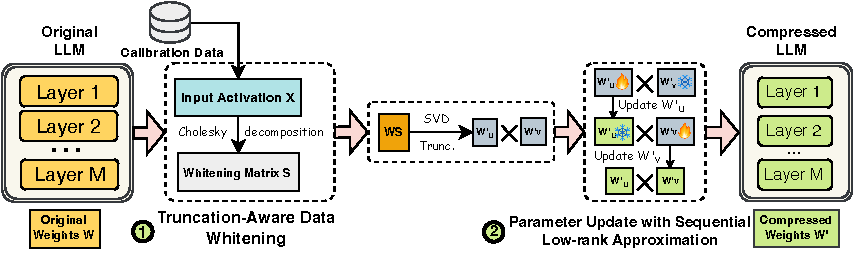
\includegraphics[width=1\textwidth]{Figures/Framework.pdf}
\vspace{-3mm}
\caption{Overview of \sysname.}
\vspace{-3mm}
\label{fig:framework}
\end{figure*}

\textbf{SVD for Language Model Compression:} Singular Value Decomposition (SVD) is a widely used low-rank approximation technique to reduce matrix size by approximating a matrix with two smaller low-ranking matrices~\citep{GOLUB1987317}. Given that, SVD is commonly used for model compression. 
%
For instance, DRONE~\citep{DBLP:conf/nips/ChenYDH21}  achieves optimal SVD compression for small language models such as BERT. However, during SVD compression, DRONE caches all the input activations, making it challenging for LLM compression due to excessive memory usage.
%, leading to the proposal of many new methods.
% %
% AAFM~\citep{DBLP:conf/aaai/YuW23} dynamically identifies the compressed model architecture and selectively compresses the output features of individual linear layers instead of the model weights. 
% %
% LoSparse~\citep{DBLP:conf/icml/LiYZLHCZ23} compresses the weight matrix by the sum of a low-rank matrix and a sparse matrix.
% %
% ARS~\citep{DBLP:conf/naacl/GaoHHSJ24} dynamically allocates the rank of the SVD compression based on the importance of weights in the LLM.
%
For LLMs, directly applying SVD on the weight matrix without considering the importance of the weights leads to a large compression loss. To address this issue, \citet{DBLP:conf/iclr/HsuHCLSJ22} propose FWSVD, which introduces Fisher information to weigh the importance of parameters. However, FWSVD requires a complex gradient calculation that demands substantial computing and memory resources for LLM compression. 
%
Another issue of directly applying SVD is that the distribution of activation can affect the compression loss. To address it, \citet{DBLP:journals/corr/abs-2312-05821} propose ASVD, which scales the weight matrix by a diagonal matrix that normalizes the impact of input channels on the weights.
%
However, both FWSVD and ASVD do not establish a direct relationship between singular values and compression loss. As a consequence, truncating the smaller singular values may lead to higher compression loss. Moreover, as compression ratio increases, it becomes necessary to update the compressed weights for accuracy recovery. However, both FWSVD and ASVD do not take it into consideration, and thus incur severe accuracy degradation under high compression ratios.

\vspace{-1mm}
\section{SVD-LLM}
\label{sec:methodology}
\vspace{-1mm}
%In this section we first present an overview of the conventional SVD compression for LLM in~\cref{subsec:conventional_SVD}. Following this, in~\cref{subsec:activation_aware_weight_whitening} and~\cref{subsec:layer_wise_close_form_update}, we present the two major modules of our SVD compression framwork, which are truncation-aware data whitening and layer-wise closed-form update. 
%
\cref{fig:framework} provides an overview of \sysname. 
%\sysname contains two main modules: (1) truncation-aware data whitening, and (2) layer-wise closed-form update. 
At a high level, \sysname is a SVD-based post-training LLM compression method.
% 
%As an overview, 
Specifically, following the standard procedure of post-training LLM compression methods~\citep{DBLP:conf/icml/FrantarA23,DBLP:journals/corr/abs-2312-05821,DBLP:conf/icml/XiaoLSWDH23},
\sysname uses a random set of sentences as calibration data to generate activation for truncation-aware data whitening. 
% before compressing LLM,  
%For the data whitening process, \sysname obtains the truncation-aware data whitening matrix through Cholesky decomposition of the multiplication of the input activation and its transpose. After whitening the input activation, \sysname performs SVD and truncates the weight matrices to compress the LLM. 
%
Given the generated activation, \sysname derives the whitening matrix $S$ through Cholesky decomposition, and then performs SVD to truncate the multiplication of weight matrices $W$ and whitening matrix $S$ to compress the LLM.
%Before outputing the compressed LLM, 
After truncation, \sysname updates the remaining model parameters with sequential low-rank approximation to recover accuracy.
%
In the following, we describe both truncation-aware data whitening and parameter update with sequential low-rank approximation in detail. The pseudocode of \sysname is provided in~\cref{appendix:pseudocode}.
%begin by discussing motivation and then provide a comprehensive illustration of each module in \sysname.




% \subsection{The Conventional SVD Compression for LLM}
% \label{subsec:conventional_SVD}
% %\begin{definition}[SVD for LLM]
% %\label{def:svd}
%     For every linear layer of LLM, suppose we use SVD to decompose its original weight matrix $W\in \mathbb{R}^{M\times N}$ with rank $r$ ($r\leq \min(M, N)$) into three matrices $U, \Sigma, V$, where $U=[u_1,u_2,u_3,...,u_r]$, $\Sigma=\text{diag}(\sigma_1,\sigma_2,\sigma_3, \cdots, \sigma_r)$, $V=[v_1,v_2,v_3,...,v_r]$. Then for the input activation $X$ with dimension $N \times n$, the output $Y$ of the forward pass can be denoted as: $Y = WX = U \Sigma V^TX = \sum_{i=1}^r \sigma_i u_i v_i^TX$. To compress $W$, we reduce its rank to $m$, where $m < r$, via only keeping the largest $m$ singular values and truncating others. In this way, we can guarantee the best approximation of $W$ with the multiplication of two small matrices $W' = W_u \cdot W_v^{T}$ where $W_u = [\sqrt{\sigma_1}u_1,\sqrt{\sigma_2}u_2,\sqrt{\sigma_3}u_3,...,\sqrt{\sigma_r}u_m]$ and $W_v=[\sqrt{\sigma_1}v_1,\sqrt{\sigma_2}v_2,\sqrt{\sigma_3}v_3,...,\sqrt{\sigma_r}v_m]$ with lowest Frobenius Loss $||W-W'||_F = \sum_{i=m+1}^r \sigma_iu_iv_i^{T}$~\citep{GOLUB1987317}.
% %\end{definition}
% \vspace{-2mm}
\subsection{Truncation-Aware Data Whitening}
% \vspace{-2mm}
%In this section, we first point out the limitations of the existing whitening solution in SVD compression as our motivation; then, we provide a detailed illustration of our own whitening strategy to solve these limitations.
\label{subsec:activation_aware_weight_whitening}
\textbf{Motivation:}
Due to high variance of input activation, simply applying vanilla SVD for LLM compression leads to severe accuracy degradation~\citep{DBLP:journals/corr/abs-2312-05821}. To address this issue, existing methods~\citep{DBLP:journals/corr/abs-2312-05821, DBLP:conf/iclr/HsuHCLSJ22} formulate LLM compression as an optimization problem with the following objective:
\vspace{-0mm}
\begin{equation}
    O = \min(||WX-W'X||_F) 
    \label{eq:t1}
\end{equation}
% \vspace{-4mm}
% \begin{align}
%      WX &= (WS)(S^{-1}X) = \tilde{W}\tilde{X} \\
%      \tilde{U}, \tilde{\Sigma}, \tilde{V} &= \text{SVD}(\tilde{W})\\
%      W'& = \tilde{U} \times \text{trunc.}( \tilde{\Sigma}) \times \tilde{V}
%     \label{eq:t1}
% \end{align}
       
where $W$ is the weight matrix of the original LLM, $X$ is the activation of $W$, $W'$ is the compressed weight matrix, and $||WX-W'X||_F$ is the compression loss in the form of Frobenius loss.

Although existing methods attempt to reduce this compression loss during their SVD truncation, they all fail to establish a direct relationship between singular values and compression loss. As a consequence, truncating smaller singular values in SVD could lead to significant compression loss. 
%
Taking ASVD~\citep{DBLP:journals/corr/abs-2312-05821} as an example, ASVD extracts a diagonal matrix $S_{0}$ from $X$ where each element in the diagonal is the absolute mean value of each channel.
%
It then uses $S_{0}$ to normalize $X$ and converts $WX$ into $(WS_{0})(S_{0}^{-1}X)$. 
%and inserts $S_{0}S_{0}^{-1}$ into the multiplication of $WX$ to , i.e, 
Subsequently, SVD is performed on $WS_{0}$ to obtain the decomposed matrices $U_{0}$, $\Sigma_{0}$, and $V_{0}$. Lastly, ASVD truncates the smallest singular values in $\Sigma_{0}$ to obtain the compressed weight matrix $W'_{0} = U_{0} \times \text{Trunc.}(\Sigma_{0}) \times V_{0} \times S_{0}^{-1}$.

%%
Although normalizing the activation improves performance, ASVD does not establish a direct relationship between singular values and compression loss (a detailed proof is included in~\cref{subsec:ASVD_reconstruction_error}).
%
To better illustrate this point, we show two concrete examples in~\cref{fig:asvd_whitening}. 
%
In example \ding{182} where only one singular value is truncated, truncating the smallest singular value 0.1 results in a higher compression loss (loss $=$ 1.1) compared to truncating the second smallest singular value 0.9 (loss $=$ 0.7). 
%
In example \ding{183} where multiple singular values are truncated, truncating the smallest two singular values 0.9 and 0.1 also leads to a higher loss (loss $=$ 1.9) than truncating 2.4 and 0.1 (loss $=$ 1.7).
%
As such, truncating the smallest singular values does not lead to minimal loss.
%Therefore, even if we have applied the data normalization method in ASVD, truncating the smallest singular values for LLM compression could still lead to higher compression loss compared to truncating larger singular values. 



%\begin{definition}[Data Whitening for SVD]
%\label{def:whitening}
    %Data whitening for SVD refers to applying an indentity mapping $I=SS^{-1}$ inside a linear layer, $Y=WSS^{-1}X$, where the whitening matrix $S^{-1}$ is designed to satisfy that the channels of the resulting activation $\tilde{X}=S^{-1}X$ are independent and have unit variance, i.e., $\tilde{X}\tilde{X}^T=I$. The subsequent SVD and compression is performed on $\tilde{W}=WS$ instead of the original weight $W$.
    % Data whitening of SVD refers to applying an invertible matrix $S$ to unify the distribution of activation $X$ for reducing the truncation loss. Suppose we have whitening matrix $S$. Denote the whitened activation as $\tilde{X}=S^{-1}X$. Then we apply SVD and truncate the singular values of $\tilde{W} = WS = \tilde{U} \tilde{\Sigma} \tilde{V}^T =\sum_{i=1}^r \tilde{\sigma}_i \tilde{u}_i \tilde{v}_i^T$. Since $Y = \tilde{W} \tilde{X}  = (W S) (S^{-1} X) = WX$, the output $Y$ does not change after whitening.
%\end{definition}

\begin{figure}[t]

\centering
\subfigure[Data Normalization (ASVD)]{
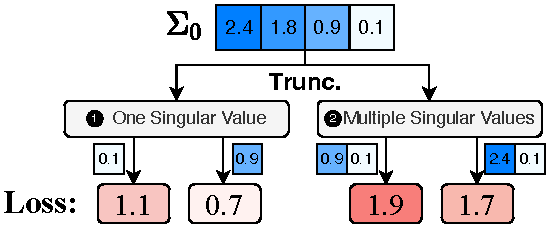
\includegraphics[width=0.45\textwidth]{Figures/white_asvd.pdf}
\label{fig:asvd_whitening}
}
\vline
\hspace{0.1cm}
\centering
\subfigure[Truncation-Aware Data Whitening (\sysname)]{
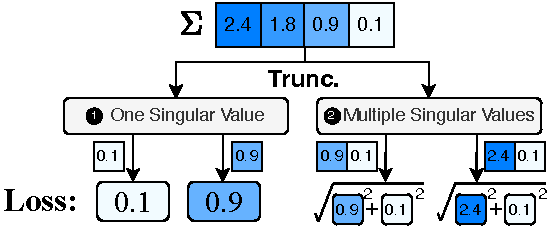
\includegraphics[width=0.45\textwidth]{Figures/white_svdllm.pdf}
\label{fig:svdllm_whitening}
}
\DeclareGraphicsExtensions.
\caption{Compression loss ($L = ||WX-W'X||_F$) of different data preprocessing methods. 
}
\vspace{-2mm}
\label{fig:whitening_comparison}
\end{figure}

\textbf{Key Design:}
The key idea of \sysname is to incorporate a truncation-aware data whitening technique that ensures a \textit{direct} mapping between singular values and compression loss. To achieve this, \sysname enforces the whitened activation $S^{-1}X$ to be orthonormal such that each channel is independent of each other, i.e., $(S^{-1}X)(S^{-1}X)^T= S^{-1}XX^T(S^{-1})^T =I$, where $S$ is derived through Cholesky decomposition~\citep{DBLP:books/siam/Meyer00}. 
%
SVD is then performed on $WS$ to obtain the decomposed matrices $U, \Sigma, V$, where $U=[u_1,u_2,u_3,...,u_r]$, $\Sigma=\text{diag}(\sigma_1,\sigma_2,\sigma_3, \cdots, \sigma_r)$, and $V=[v_1,v_2,v_3,...,v_r]$. Lastly, the smallest singular values in $\Sigma$ are truncated (denoted by $\boldsymbol{\operatorname{Trunc.}}(\Sigma)$) to obtain two low-ranking matrices $W'_u = U\times [\boldsymbol{\operatorname{Trunc.}}(\Sigma)] ^\frac{1}{2}, W'_v = [\boldsymbol{\operatorname{Trunc.}}(\Sigma)] ^\frac{1}{2}\times  V^T \times S^{-1}$ and the compressed weight matrix $W' = W'_u \times W'_v = U \times \boldsymbol{\operatorname{Trunc.}}(\Sigma) \times V^T \times S^{-1}$. 
%
% {\color{red} 
% To save model memory, \sysname replace the original matrix $W$ with the two smaller and low-ranking ones $W_u = U\times [\boldsymbol{\operatorname{Trunc.}}(\Sigma)] ^\frac{1}{2}, W_v = [\boldsymbol{\operatorname{Trunc.}}(\Sigma)] ^\frac{1}{2}\times  V^T \times S^{-1}$ in the compressed LLM.
% }

%%
\cref{fig:svdllm_whitening} illustrates the effect of the proposed truncation-aware data whitening method. In example \ding{182} where only one singular value is truncated, the compression loss equals to the truncated singular value. In example \ding{183}, the compression loss of truncating multiple singular values equals to the square root of the sum of their squares. As such, under the proposed truncation-aware data whitening technique, truncating the smallest singular values leads to minimal compression loss.

%%
In the following, we provide a theoretical proof on why the proposed  truncation-aware data whitening technique ensures a direct mapping between singular values and compression loss in the case of one singular value (\cref{thm:whitening}) and multiple singular values (\cref{col:whitening}), respectively.

\vspace{0mm}
\begin{lemma}
\label{lem:frobenius}
    The Frobenius norm of matrix $A$ with dimension $m\times n$ can be deduced into the square root of the trace of its gram matrix, which is: 
        \begin{equation}
        \|A\|_F \triangleq\left(\sum_{j=1}^n \sum_{i=1}^m\left|a_{i j}\right|^2\right)^{\frac{1}{2}} =\left[\boldsymbol{\operatorname{Trace}}\left(A^T A\right)\right]^{\frac{1}{2}}
        \end{equation}
\end{lemma}
% \vspace{-3mm}
Let $\boldsymbol{\operatorname{SVD}}(WS)$ denote SVD compression on matrix $WS$. The compressed weight matrix $W'$ can be expressed as $W' = \boldsymbol{\operatorname{SVD}}(WS)S^{-1}$. Using \cref{lem:frobenius}, we obtain the compression loss $L_i$ when truncating the $i^{th}$ singular value of $WS$ to reduce its rank for compression:
\begin{equation}
\label{formula:loss}
    \begin{split}
    L_i&=\left\|W X-W^{\prime} X\right\|_F=\left\|W S S^{-1} X-\boldsymbol{\operatorname{SVD}}(W S) S^{-1} X\right\|_F=\left\|(W S-\boldsymbol{\operatorname{SVD}}(W S)) S^{-1} X\right\|_F\\
    &=\left\|\sigma_i u_i v_i^T S^{-1} X\right\|_F=\sigma_i \boldsymbol{\operatorname{Trace}}\left(u_i v_i^T S^{-1} X X^T\left(S^{-1}\right)^T v_i u_i^T\right)^{\frac{1}{2}}
    \end{split}
\end{equation}
Since both $U=[u_1,u_2,u_3,...,u_r]$ and $V=[v_1,v_2,v_3,...,v_r]$ are orthonormal matrices, we have:
\begin{equation}
v_i^T v_i = u_i^T u_i = 1; v_i^T v_j = u_i^T u_j = 0, \forall i \neq j ; \boldsymbol{\operatorname{Trace}}(v_i v_i^T) = \boldsymbol{\operatorname{Trace}}(u_i u_i^T) =1
\end{equation}

\begin{theorem}
\label{thm:whitening}
If $S$ is the Cholesky decomposition of $XX^T$, the compression loss $L_i$ equals to $\sigma_i$.
\end{theorem}
% \vspace{-2mm}
\begin{proof}
\label{proof:whitening}
Since the whitening matrix $S$ is the Cholesky decomposition of $XX^T$, we have $SS^T=XX^T$. We can further infer \cref{formula:loss} to obtain:
\begin{equation}
L_i = \sigma_i \boldsymbol{\operatorname{Trace}}(u_i v_i^T v_i u_i^T)^{\frac{1}{2}} = \sigma_i \boldsymbol{\operatorname{Trace}}\left(u_i\left(v_i^T v_i\right) u_i^T\right)^{\frac{1}{2}}=\sigma_i \boldsymbol{\operatorname{Trace}}\left(u_i u_i^T\right)^{\frac{1}{2}} = \sigma_i \\
\end{equation}
Therefore, $L_i$ of truncating $\sigma_i$ equals to the singular value $\sigma_i$ itself.
\end{proof}
\begin{corollary}
\label{col:whitening}
If $S$ is the Cholesky decomposition of $XX^T$, truncating the smallest singular values leads to the lowest loss $L$ compared to truncating others.
\end{corollary}

% \vspace{-3mm}
\begin{proof}
\label{proof:truncation}
If we truncate $\sigma_{m+1}, \sigma_{m+2}, \sigma_{m+3},..., \sigma_{r}$ in $\Sigma$ for compression, the square of the loss $L$ is:
\begin{equation}
    \begin{split}
    L^2 =& \left|\left| \sum_{i=m+1}^r \sigma_i u_i v_i^T S^{-1}X \right|\right|^2_F =\sum_{j=m+1}^r\sum_{i=m+1}^r\sigma_i\sigma_j\boldsymbol{\operatorname{Trace}}(u_i v_i^T S^{-1}XX^T(S^{-1})^T v_j u_j^T) \\
=& \sum_{i=m+1}^r\sigma_i^2\boldsymbol{\operatorname{Trace}}(u_i v_i^T S^{-1}XX^T(S^{-1})^T v_i u_i^T) = \sum_{i=m+1}^r(L_i )^2=\sum_{i=m+1}^r(\sigma_i)^2
    \end{split}
\end{equation}
The squared loss $L^2$ equals to the sum of the squared singular values (More detailed derivation is in Appendix~\ref{appendix:compression_loss_svdllm}). Truncating the smallest singular values achieves the lowest compression loss.
\end{proof}

%
Given that our proposed truncation-aware data whitening technique is built upon SVD, whose applicability depends on certain singular value distribution, we further conduct a spectrum analysis of the singular values obtained by our technique. We refer the readers to Appendix~\ref{appendix:spectrum_analysis} for details.

%
It should also be noted that our proposed truncation-aware data whitening technique not only ensures a direct mapping between singular values and compression loss, but is also able to achieve the same theoretical optimal compression loss as DRONE~\citep{DBLP:conf/nips/ChenYDH21}.
%
%Apart from aligning the SVD truncation with the compression loss, our data whitening method can even achieve the minimum compression loss, as been done in previous work DRONE~\citep{DBLP:conf/nips/ChenYDH21} on small LMs. 
%
However, during SVD compression, DRONE stores all input activations in memory, which poses a challenge for LLM compression due to high memory consumption.
%However, due to the requirement of caching all input activations, DRONE is difficult to be applied for LLM compression due to significant memory consumption. 
%
In contrast, \sysname incrementally updates its $XX^T$ matrix by adding the $xx^T$ of each new input $x$,  which is considerably smaller than the full input activation.
%
In~\cref{appendix:comparison_with_drone}, we provide our proof on \sysname achieving the same theoretical optimal compression loss as DRONE and discuss the advantages of \sysname over DRONE in memory saving, compression speed, and numerical stability in details.
%Compared with DRONE, SVD-LLM makes improvements in terms of memory, speed, and numerical stability. 
%More detailed analysis about the optimality of \sysname and comparison with DRONE are provided in~\cref{appendix:comparison_with_drone}.


% \vspace{-3mm}
% \subsection{Layer-Wise Closed-Form Update}
% \label{subsec:layer_wise_close_form_update}
% \textbf{Motivation:}
% Given the same calibration data as input, the compressed weight matrix $W'$ generates a new activation $X'$ that is different from $X$ generated by the original weight matrix $W$. As the compression ratio increases, $W$ needs to truncate a larger number of singular values to obtain $W'$, thus $X'$ deviates further from $X$. Therefore, it becomes necessary to design a strategy for updating $W'$ to minimize $||WX'-W'X'|| _F$. However, existing SVD-based LLM compression methods have no design of parameter update after compression, leading to less competitive performance at high compression ratios.

% \begin{wrapfigure}{r}{0.45\textwidth} % "r" 表示右侧，"0.5\textwidth" 控制宽度
%   \centering
%   \vspace{-5mm}
%   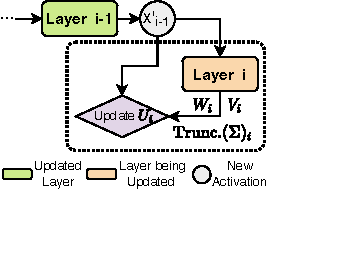
\includegraphics[width=0.31\textwidth]{Figures/updating_strategy_1.pdf} % 调整图像大小
%   \caption{Layer-Wise Closed-Form Update.}
%    \label{fig:local_update}
% \end{wrapfigure}
% \textbf{Key Design:}
% %
% The key idea of \sysname is to incorporate a layer-wise closed-form strategy to update $W'$ to minimize $||WX'-W'X'|| _F$. \cref{fig:local_update} illustrates the overall process. To perform the update in layer $i$, \sysname uses the new activation $X'_{i-1}$ from the previous layer $i-1$ that has been updated. To perform the update without destroying the low-rank structure of $W'_{i}$, \sysname only updates the matrix $U_{i}$ to its closed-form solution $U'_i$ while keeping $\text{Trunc.}(\Sigma)_i$ and $V_i$ fixed as: 
% \begin{equation}
% \label{eq:close_form}
%     \begin{split}
%     % U_i' = \arg \min_{U'} || WX' - W'X'||_F = \arg \min_{U'} || WX' - U'\Sigma_1 V^T S^{-1}X'||_F
%     U_i' &= \arg \min_{U_i} || W_i X'_{i-1} - W'_i X'_{i-1}||_F \\
%     &=  \arg \min_{U_i} || W_i X'_{i-1} - U_i \text{Trunc.}(\Sigma)_i \times V_i^T \times S_i^{-1}X'_{i-1}||_F\\
%     &= W_i X'_{i-1} D^T (D D^T)^{-1}, \text{where } D = \text{Trunc.}(\Sigma)_i V_i^TS_i^{-1} X'_{i-1}
%     \end{split}
% \end{equation}
% \vspace{-3mm}

\subsection{Parameter Update with Sequential Low-rank Approximation}
\label{subsec:lora_finetunig}
\textbf{Motivation:} 
%
Although the proposed truncation-aware data whitening technique helps preserve the accuracy during compression, as the compression ratio increases, the accuracy of the compressed LLM may degrade given that more larger singular values will be truncated by SVD compression.
% Although the truncation-aware data whitening method helps \sysname to reduce the compression loss in each layer of LLMs, this layer-wise compression, which has been commonly applied in many post-training LLM compression works, is difficult to ensure the global minimization of the performance drop of the compressed LLM, especially under the high compression ratio. 
% % As we can see in Figure xxx, when the compression ratio is higher than 0.5, indicating that more than 50\% of the parameter reduction, the perplexity of the compressed LLM drops significantly. 
Therefore, it is necessary to update the remaining parameters in the compressed LLM.


\textbf{Key Design:} 
%
%Driven by previous post-training LLM compression works~\citep{DBLP:conf/nips/MaFW23}, 
\sysname proposes a variant of LoRA fine-tuning to update the remaining weight parameters of the compressed LLM for accuracy recovery. 
%
Specifically, given the two low-ranking matrices $W'_u, W'_v$ generated by truncation-aware data whitening,
%, as discussed in the pseudocode in Appendix~\ref{appendix:pseudocode}. 
%which would break its low-rank structure, 
instead of directly applying LoRA fine-tuning to the compressed weight matrix $W' = W'_u\times W'_v$ as standard LoRA does, we propose to apply LoRA on top of $W'_u$ and $W'_v$ separately to preserve their low-rank structures as follows:
\begin{align}
    W'_u \leftarrow W'_u + B_uA_u, W'_v\leftarrow W'_v + B_vA_v
\end{align}
where $A_u$, $B_u$, $A_v$, and $B_v$ are matrices used for LoRA fine-tuning. 

%
Simultaneously fine-tuning $W'_u$ and $W'_v$ will not guarantee a decrease in fine-tuning loss. This is because the derivatives of $W'_u$ and $W'_v$ are interdependent during the fine-tuning process, where optimization of one matrix may interfere with the optimization of the other. 
%As a result, the overall effect on the fine-tuning loss function may not always lead to a reduction in loss. 
%
Therefore, as shown in Figure~\ref{fig:framework}, we propose a sequential low-rank approximation strategy to fine-tune $W'_u$ and $W'_v$ in a sequential manner. 
%
Specifically, we first freeze matrix $W'_v$ and fine-tune $W'_u$ with LoRA. We then perform the second-round LoRA fine-tuning on matrix $W'_v$ while freezing the updated weight matrix $W'_u$. Finally, we add $B_u\times A_u$ and $B_v\times A_v$ matrices to $W'_u$ and $W'_v$ to obtain the final compressed weight matrices.


\section{Experiments and Analysis}
\label{sec:experiments}
\vspace{-1mm}
%\subsection{Experimental Setups}
%\label{subsec:setup}

%%
\textbf{Baselines.}
%
We compare \sysname against three groups of methods: (1) Vanilla SVD and state-of-the-art SVD-based LLM compression methods: FWSVD~\citep{DBLP:conf/iclr/HsuHCLSJ22}, ASVD~\citep{DBLP:journals/corr/abs-2312-05821} (Section~\ref{subsec:overall_performance}) and FLAP (\cref{appendix:flap_comparison}).
%
(2) Other types of LLM compression methods. These include three state-of-the-art pruning-based LLM compression methods: LLM-Pruner~\citep{DBLP:conf/nips/MaFW23}, SliceGPT~\citep{DBLP:conf/iclr/AshkboosCNHH24}, and BlockPruner~\citep{DBLP:journals/corr/abs-2406-10594}, and three state-of-the-art quantization-based LLM compression methods: PB-LLM~\citep{DBLP:conf/iclr/YuanSD24}, BiLLM~\citep{DBLP:conf/icml/HuangLQLZ0M024}, and OneBit~\citep{DBLP:conf/nips/Xu0YWZLLC24} (Section~\ref{subsection:Comparison_with_other_compression_methods}). 
%
(3) Smaller LLM StableLM-3B~\citep{StableLM-3B-4E1T} pre-trained from scratch (\cref{appendix:pretrained_comparison}).

\textbf{Models and Datasets.} 
%
To demonstrate the generability of \sysname, we evaluate the performance of \sysname on seven models from three different LLM families at three different scales (LLaMA-7B, 13B, 30B, LLaMA2-7B~\citep{DBLP:journals/corr/abs-2307-09288}, OPT-6.7B~\citep{DBLP:journals/corr/abs-2205-01068}, Vicuna-7B~\citep{vicuna2023} and Mistral-7B~\citep{DBLP:journals/corr/abs-2310-06825}) and $10$ datasets including two language modeling datasets (WikiText-2~\citep{DBLP:conf/iclr/MerityX0S17}, and C4~\citep{DBLP:journals/jmlr/RaffelSRLNMZLL20}), six classification datasets (OpenbookQA~\citep{DBLP:conf/emnlp/MihaylovCKS18}, WinoGrande~\citep{DBLP:conf/aaai/SakaguchiBBC20}, HellaSwag~\citep{DBLP:conf/acl/ZellersHBFC19}, Arc\_e~\citep{DBLP:journals/corr/abs-1803-05457}, PIQA~\citep{DBLP:conf/aaai/BiskZLGC20}, MathQA~\citep{DBLP:conf/naacl/AminiGLKCH19}),  and two generation datasets (TruthfulQA~\citep{DBLP:conf/acl/LinHE22} and GSM8K~\citep{DBLP:journals/corr/abs-2110-14168}) with the LM-Evaluation-Harness framework~\citep{eval-harness}.

%
\textbf{Implementation Details.}
%
To ensure a fair comparison, we followed ASVD~\citep{DBLP:journals/corr/abs-2312-05821} to randomly select 256 samples from WikiText-2 as the calibration data. 
We followed the same configuration used in LLM-Pruner~\citep{DBLP:conf/nips/MaFW23} to use Alpaca~\citep{alpaca} dataset with 50K samples for parameter update in \sysname.
% All of our experiments are conducted on NVIDIA A100 GPUs.
The inference efficiency experiment is conducted on both NVIDIA A100 GPU and AMD EPYC 7643 CPU while the other experiments are conducted on NVIDIA A100 GPUs.
%Due to page limit, implementation details are provided in~\cref{appendix:experimental_setup}.

%%Compression Accuracy Analysis
\vspace{-2mm}
\subsection{Comparison with State-of-the-Art SVD-based LLM compression Methods}
\label{subsec:overall_performance}
\vspace{-2mm}
First, we compare the performance of \sysname with state-of-the-art SVD-based LLM compression methods from four aspects: (1) performance under different compression ratios, (2) performance on different LLMs, (3) performance on LLMs with larger scales, and (4) compression speed (\cref{appendix:compression_speed}). 
%
Given that all the SVD-based baselines do not incorporate LoRa fine-tuning, to ensure a fair comparison, we also compare to 
\sysname with truncation-aware data whitening only (denoted as \sysname \texttt{(W)}).

\accuracyTable
\differntllmaccuracyTable
\textbf{Performance under Different Compression Ratios.}
We first evaluate the performance of LLaMA-7B compressed by \sysname, \sysname \texttt{(W)}, and the SVD-based baselines under compression ratios ranging from 20\% to 80\% on all $10$ datasets. 
%
The results are summarized in\cref{tab:dataset_acc}. Both \sysname and \sysname \texttt{(W)} consistently outperform vanilla SVD, FWSVD and ASVD across all the compression ratios. In particular, when the compression ratio is 40\% and above, \sysname reduces the perplexity by more than 99\% on two language modeling datasets and achieves over 400\% higher average accuracy on six classification datasets. More importantly, the results on two generation datasets (TruthfulQA, GSM8K) of all three baselines when compression ratios are 60\% and above are zero, meaning that the compressed LLMs totally lose their generation ability. In contrast, \sysname still outputs good generation even under 80\% compression ratio. 
%
Example contents generated by the compressed LLMs are included in~\cref{sec:appendix_example}.
%
%These results indicate that \sysname is more effective in compressing LLMs for more resource-constrained devices such as smartphones and IoT devices.

%%


\begin{wrapfigure}{r}{0.48\textwidth} % "r" 表示右侧，"0.5\textwidth" 控制宽度
  \centering
  \vspace{-5mm}
  \largellmaccuracyTable
\end{wrapfigure}

\textbf{Performance on Different LLMs.} To examine the generability of \sysname and \sysname \texttt{(W)} across different LLMs, we compare the performance between \sysname and the baselines on four different models from three different LLM families -- OPT-6.7B (OPT family), LLaMA 2-7B (LLaMA family), Mistral-7B (Mistral family), and Vicuna-7B (LLaMA family)  -- under 20\% compression ratio on WikiText-2 and six classification datasets. 
%
As shown in~\cref{tab:different_llm_acc}, both \sysname and \sysname \texttt{(W)} consistently outperform baselines on all four LLMs, and exhibits more stable performance across different LLMs, especially compared to vanilla SVD and FWSVD.

\textbf{Performance on LLMs with Larger Scales.} To examine the generability of \sysname and \sysname \texttt{(W)} on LLMs with larger scales, we compare the performance between \sysname and the baselines on LLaMA-13B and LLaMA-30B under 20\% compression ratio. As shown in~\cref{tab:large_llm_acc}, both \sysname and \sysname \texttt{(W)} consistently outperform vanilla SVD, FWSVD, and ASVD on both model sizes. 


\vspace{-1mm}
\subsection{Inference Efficiency of \sysname }
\label{subsec:inference_speedup}
\vspace{-1mm}
% Next, to illustrate the inference speedup and memory reduction of LLMs compressed by \sysname, we provide theoretical analysis as well as empirical evaluation on real-world hardware.

\textbf{Theoretical Analysis of Inference Efficiency.} Assume \sysname compresses the weight matrix {\small$W \in \mathbb{R}^{d \times n}$} into two low-ranking matrices {\small$W_u' \in \mathbb{R}^{d \times r}, W_v' \in \mathbb{R}^{r \times n}$}. The compression ratio is then calculated as {\small$R_w = 1-\frac{(d+n) r}{d n}$}.

\underline{(1) Compute Complexity Analysis:} Given input {\small$X \in \mathbb{R}^{n \times d}$}, instead of recalculating the full weight matrix {\small$W^{\prime}=W_u' \times W_v'$} and then computing the output {\small$W^{\prime} \times X$}, \sysname calculates the intermediate state {\small$M=W_v' \times X$} and then computes the output {\small$Y=W_u' \times M$}. 
%
In this way, the computation complexity is reduced from {\small$O\left(d^2 n\right)$} to {\small$O\left(d^2 r+r n d\right)$}. 
%
Taking compression ratio {\small$R_w=50\%$} as an example, since {\small$R_w=1 - \frac{(d+n) r}{d n}$}, we have {\small$r=\frac{d n}{2(d+n)}$}. Then the computation complexity is
{\small$O\left(d^2 r+r n d\right)=O(r d(d+n))=O\left(\frac{d^2 n}{2}\right)=\frac{1}{2} O\left(d^2 n\right)$}, which reduces {\small$50\%$}. In general, given any compression ratio $R_w$, the computation complexity is reduced to {\small$1 - R_w$} times of the original.

\begin{figure}[htbp]
 \vspace{-0mm}
     \begin{minipage}{0.98\textwidth}
     \centering
    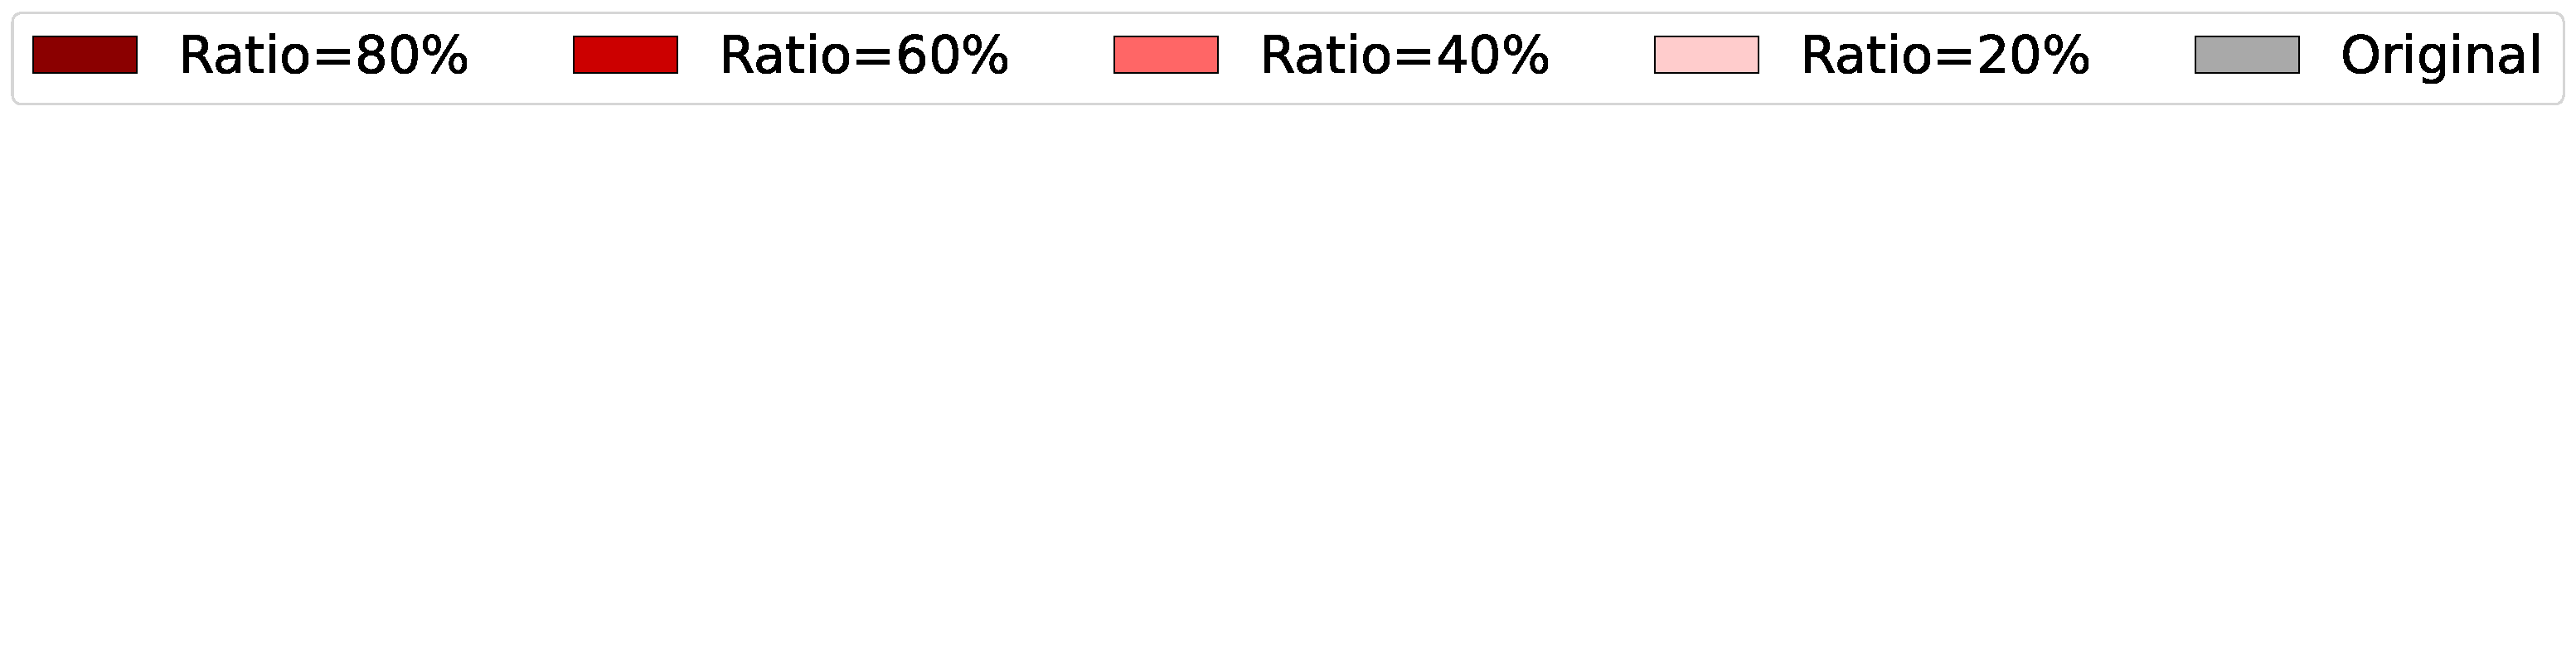
\includegraphics[width=1\linewidth]{Figures/legend.pdf}
     \end{minipage}
     \\
     \begin{minipage}{1\textwidth}
        \subfigure[Varying Batch Size on GPU]{
            \centering
            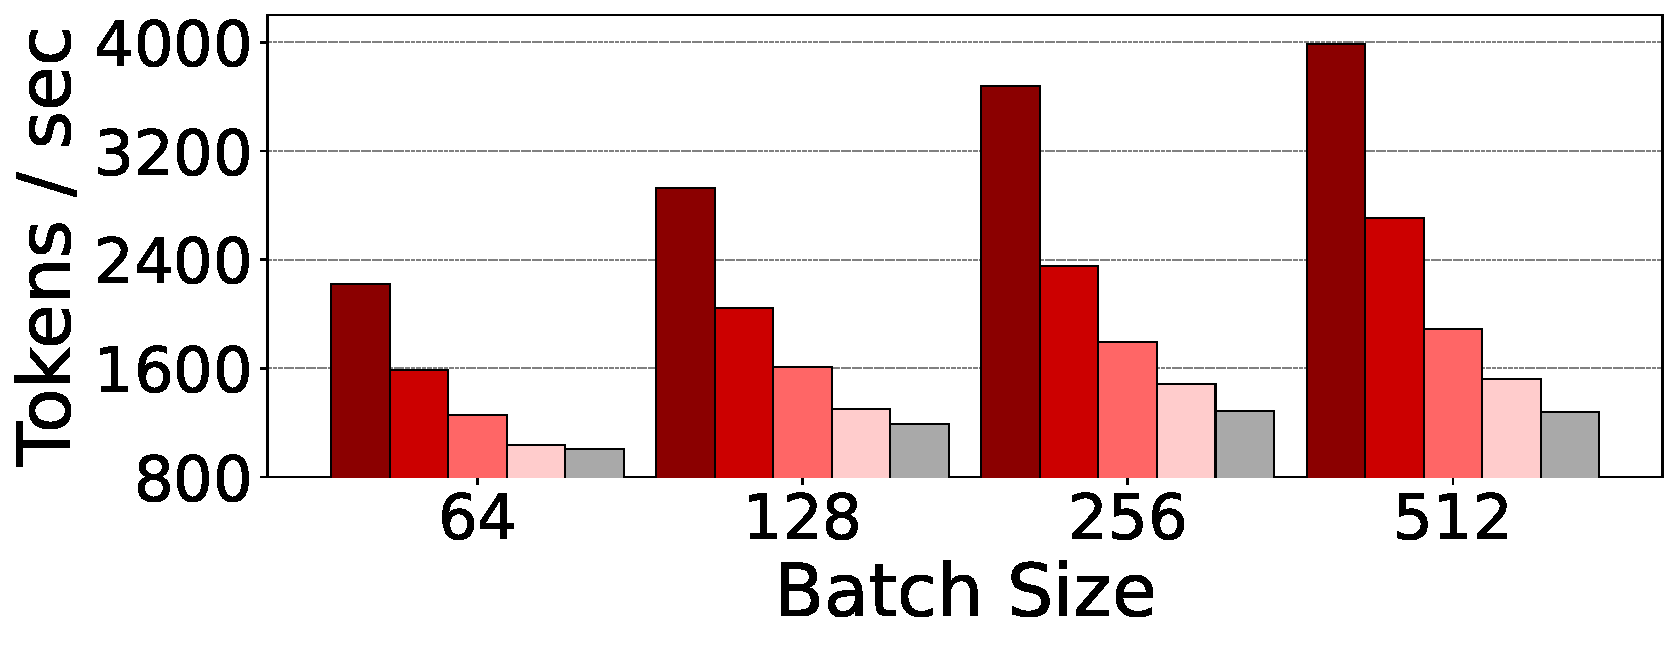
\includegraphics[width=0.48\textwidth]{Figures/eff_bs_gpu.pdf}
            \label{fig:bs_gpu}
            }
        \subfigure[Varying Sequence Length on GPU]{
            \centering
            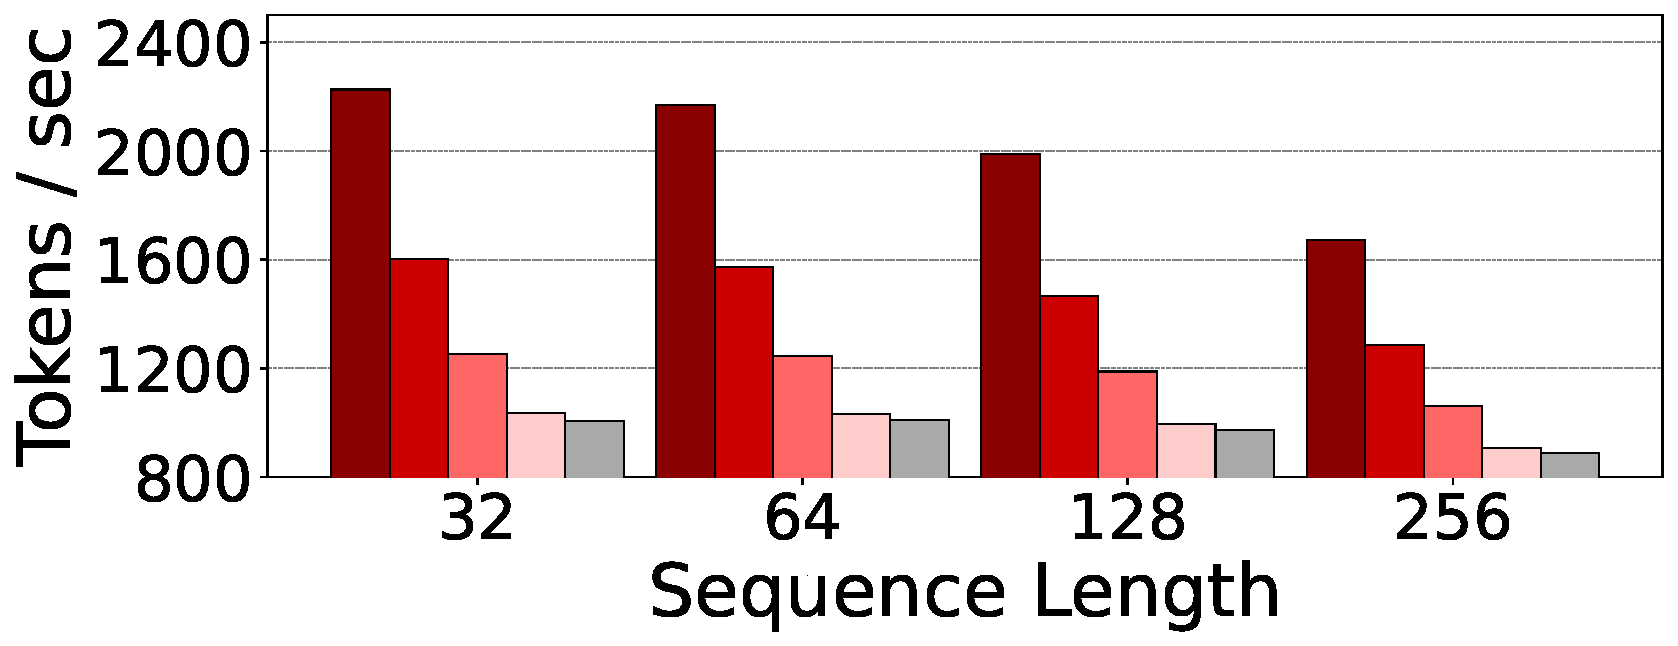
\includegraphics[width=0.48\textwidth]{Figures/eff_sl_gpu.pdf}
            \label{fig:sl_gpu}
            }
        \\
        \subfigure[Varying Batch Size on CPU]{
            \centering
            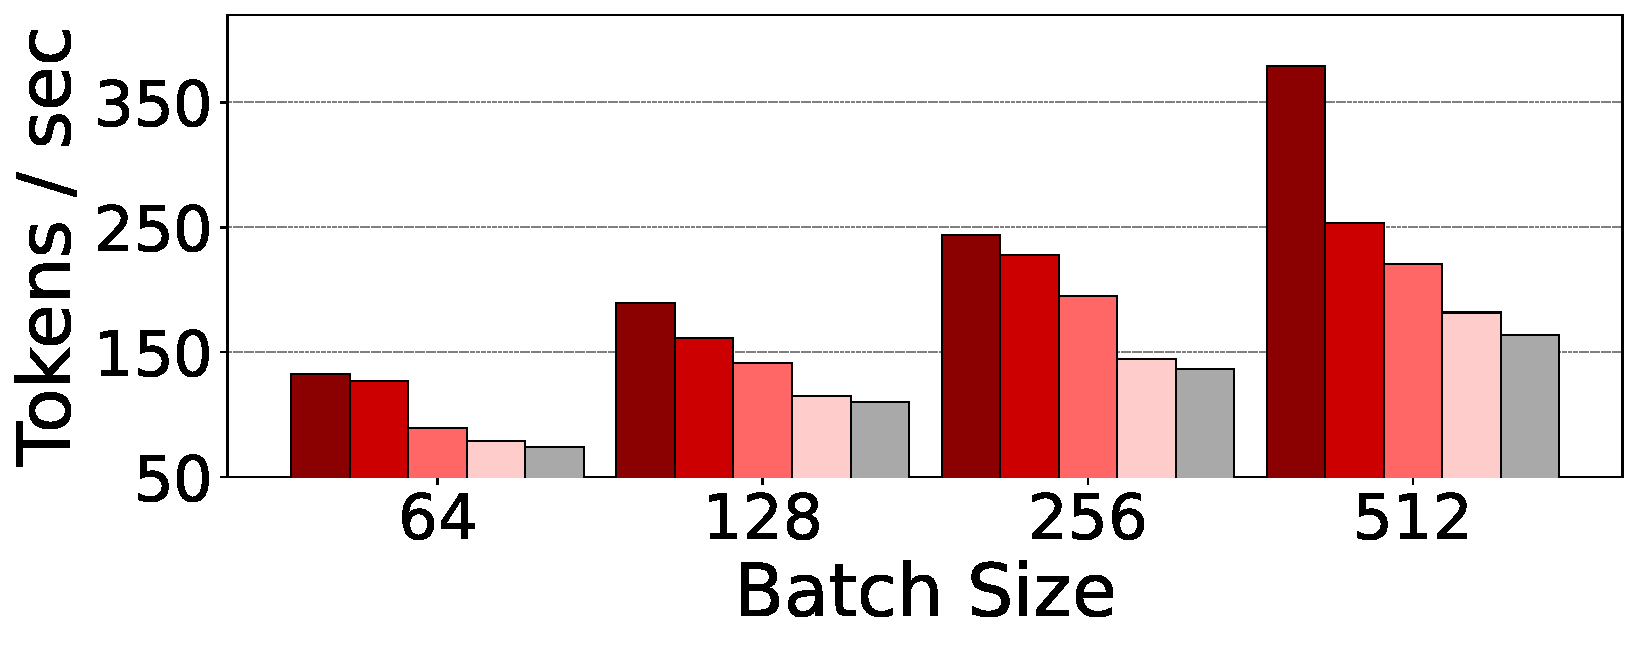
\includegraphics[width=0.48\textwidth]{Figures/eff_bs_cpu.pdf}
            \label{fig:bs_cpu}
            }
        \subfigure[Varying Sequence Length on CPU]{
            \centering
            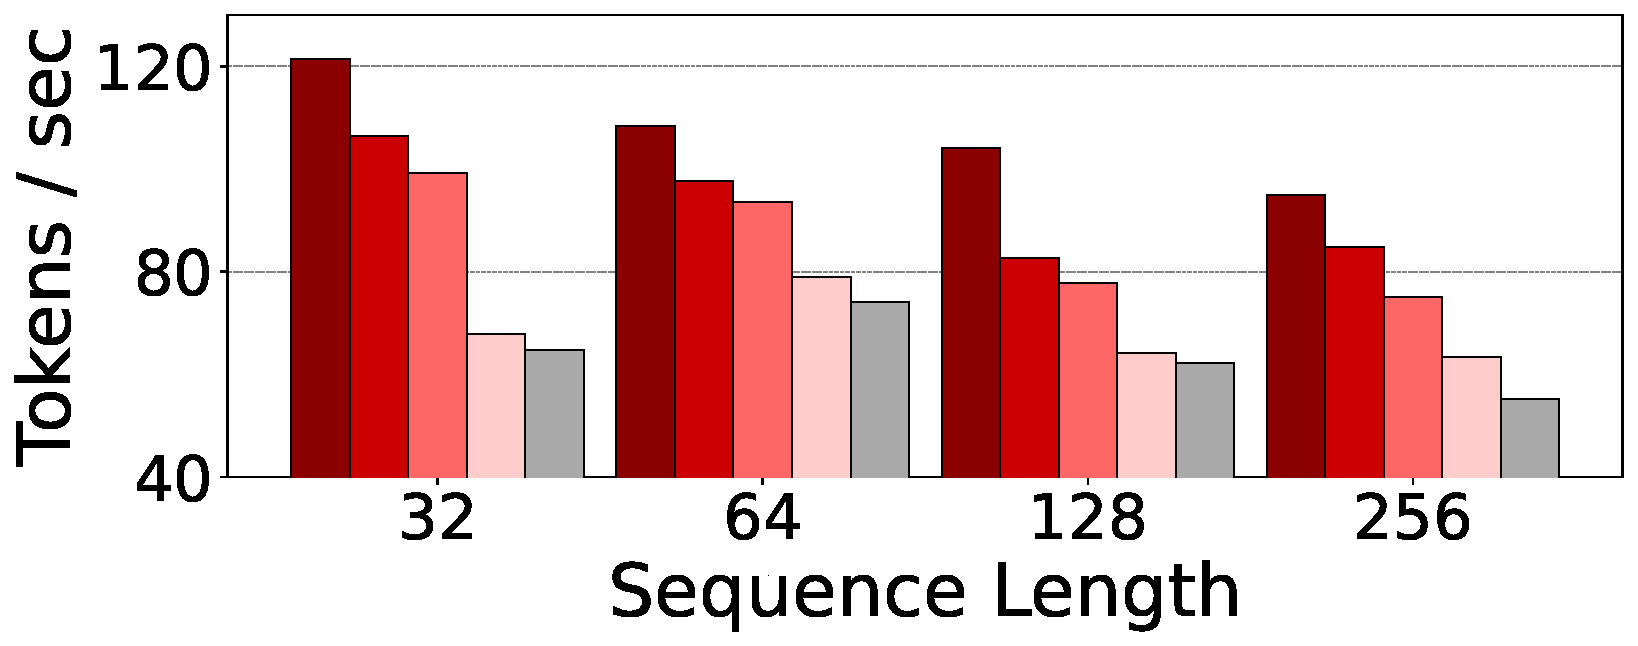
\includegraphics[width=0.48\textwidth]{Figures/eff_sl_cpu.pdf}
            \label{fig:sl_cpu}
            }
        \DeclareGraphicsExtensions.
        \vspace{-2mm}
        \caption{Throughput (tokens/sec) of LLaMA-7B and its compressed version by \sysname under different compression ratios on a single A100 GPU under different batch sizes (a) and different sequence lengths (b) and on a single AMD EPYC 7643 CPU under different batch sizes (c) and different sequence lengths (d). For (a) and (c), sequence length is 32. For (b) and (d), batch size is 64.}
        \vspace{-2mm}
        \label{fig:gpu_throughput}
    \end{minipage}
\end{figure}

\underline{(2) Inference Memory Analysis:} 
%
Since \sysname does not recalculate the full weight $W^{\prime}=W_u' \times W_v'$, the weight memory is reduced to $1 - R_w$ times of the original during inference.
%
As another advantage, \sysname is able to reduce the runtime KV cache memory as well~\citep{DBLP:journals/corr/abs-2406-13035, wan2025meda,DBLP:journals/corr/abs-2409-09808}. Specifically, instead of keeping {\small$W_u' \times W_v' \times X$} in the KV cache, \sysname provides the option to store the intermediate result {\small$M=W_v' \times X$} in the KV cache and recomputes the original key and value states with the decomposed weight matrix {\small$W_u'$} if required. As such, the runtime KV cache is reduced to {\small$\frac{r}{d}= (1 - R_w)\times \frac{d}{n+d}$} times of the original. Moreover, since {\small$W_u'$} is already stored as the weight matrix in the decomposed LLM, the original intermediate state matrix can still be recovered by {\small$W_u'\times M$} without accuracy drop. Therefore, \sysname provides a unified solution that enables \textit{simultaneous} model compression and KV cache compression.
%into a single process. 
% This is different from existing quantization or parameter pruning-based LLM compression methods that need to be combined with other techniques for compressing both weights and KV cache. 


\textbf{Inference Speedup on Hardware.} 
%
To quantify inference speedup achieved by \sysname on real hardware, we measure the numbers of tokens that LLaMA-7B and its compressed version by \sysname generate per second (i.e., throughput) under different batch sizes and sequence lengths on a single NVIDIA A100 GPU and a single AMD EPYC 7643 CPU, respectively. 
%
The results are shown in~\cref{fig:gpu_throughput}. We have three observations. 
%
(1) Under a specific batch size or sequence length, the speedup achieved by \sysname related to the original model increases as the compression ratio increases.
%consistently enhances the token generation speed across all the compression ratios. 
%
(2) Under a specific compression ratio, the speedup  achieved by \sysname related to the original model becomes more significant as the batch size increases or as the sequence length decreases.
%
(3) The above two observations are valid for both GPU and CPU.
%resulting in a maximum speedup of 1.2x on GPU and 1.1x on CPU under 20\% compression ratio, 1.7x on GPU and 1.5x on CPU under 40\% compression ratio, 2.1x on GPU and 1.64x on CPU under 60\% compression ratio, and 3.1x on GPU and 2.3x on CPU under 80\% compression ratio. 
%These results highlight the effectiveness of \sysname in enhancing the inference efficiency of LLMs on real hardware.


\textbf{Inference Memory Reduction on Hardware.} 
% \sysname is able to compress not only LLMs but also the runtime KV cache \textit{at the same time}.
Lastly, we evaluate the inference memory saving, including both weight memory and runtime KV cache memory saving on a single A100 GPU. 
%
Specifically, we measure the peak memory footprint during inference when generating 128 tokens with batch size of 32 using LLaMA-7B compressed by \sysname under different compression ratios w/ and w/o considering KV cache reduction. 
%
The results are illustrated in~\cref{fig:kv} where the memory reduction from the dotted line to the blue bars comes mainly from model weight compression and the memory reduction from the blue bars to the yellow bars comes mainly from KV cache compression. 
%
As shown, both weight memory saving and runtime KV cache memory saving brought by \sysname are near linear to the compression ratio.
%, which aligns with our theoretical analysis. 
%In particular, \sysname is able to save additional 51\% memory from its KV cache under 80\% compression ratio.


\begin{figure}[htbp]
\vspace{-5mm}
    \centering
    \begin{minipage}{0.5\textwidth}
    \centering
    \vspace{4mm}
        \centering
        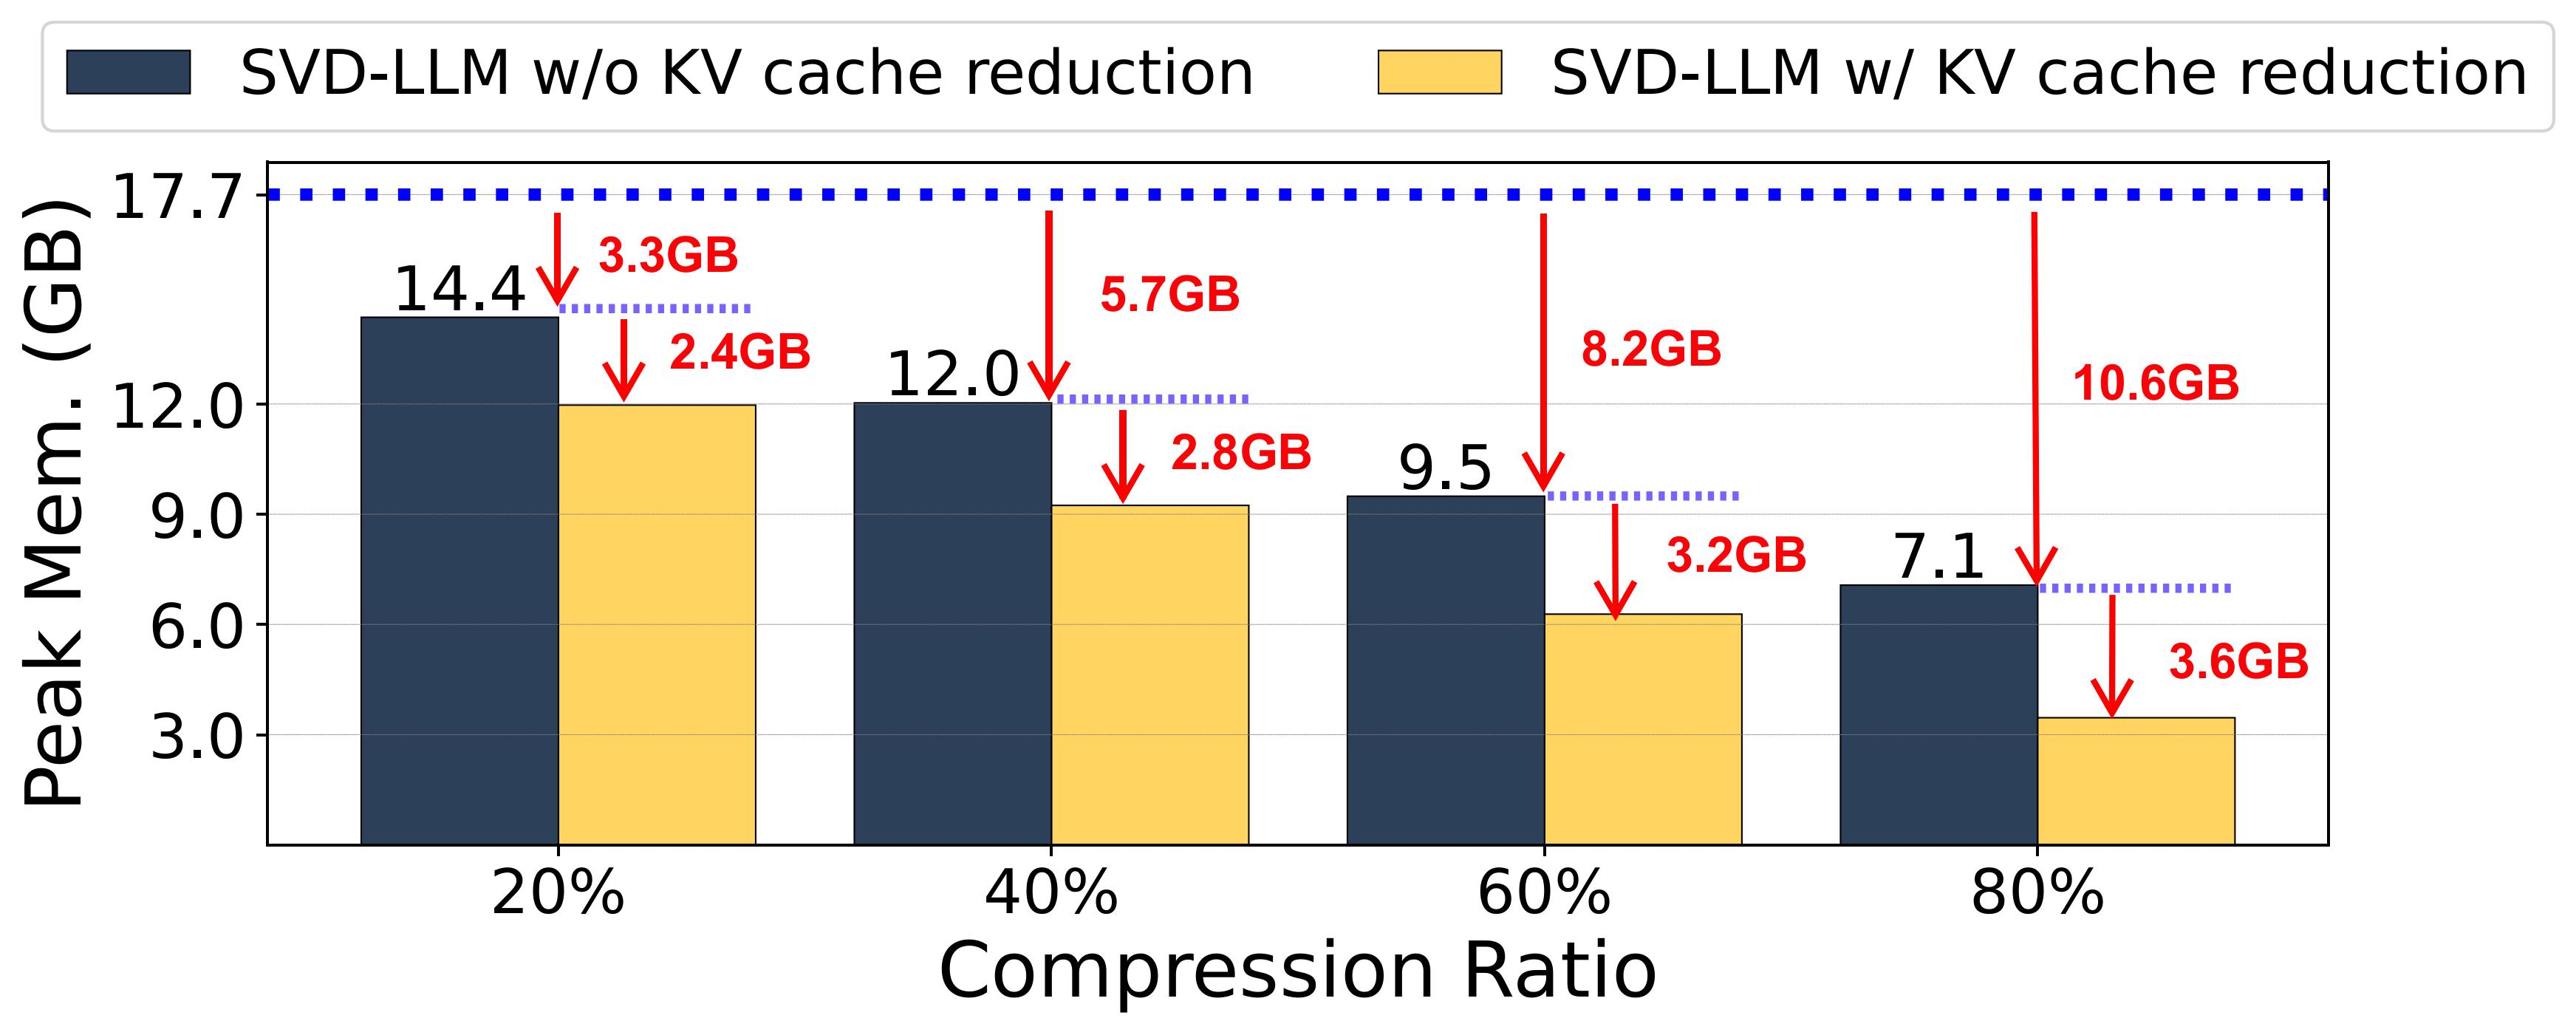
\includegraphics[width=1\textwidth]{Figures/kv_bs_1.jpg}
        \vspace{-5mm}
        \caption{Peak memory to generate 128 tokens with batch size of 32 using LLaMA-7B compressed by \sysname w/ and w/o KV-cache reduction. The dotted line indicates the peak memory of the original LLaMA-7B. The memory reduction from the dotted line to the blue bars mainly comes from the model compression. The memory reduction from the blue to the yellow bars mainly comes from the reduced footprint of the KV cache.}
        \label{fig:kv}
    \end{minipage}%
    \hspace{0.1cm}
    \begin{minipage}{0.485\textwidth}
    \centering
    \sensitivityTable
\end{minipage}
\vspace{-3mm}
\end{figure}

\vspace{-1mm}
\subsection{Ablation Study}
\label{subsec:ablation_study}
\vspace{-1mm}

%\xin{In this section, we provide three ablation studies of \sysname while more are provided in~\cref{appendix:more_ablation} due to page limit.}
%%
% 

\textbf{Modular Sensitivity Study.}
% \vspace{-2mm}
We conduct ablation studies to evaluate the separate contributions of the two key components (i.e., truncation-aware data whitening and parameter update with sequential low-rank approximation) of \sysname. 
%
Let \sysname \texttt{(W)} denote the version of \sysname with truncation-aware data whitening only; \sysname \texttt{(U)} denote the version of \sysname with \xin{normal SVD truncation} and parameter update with sequential low-rank approximation.
%; and \sysname  denote the version of \sysname with both truncation-aware data whitening and parameter update with sequential low-rank approximation.
As shown in~\cref{tab:sensitivity}, we have three observations. 
%
(1) \sysname\texttt{(W)}, \sysname\texttt{(U)} and \sysname  consistently outperform ASVD across all the compression ratios. Notably, when the compression ratio is at and above 40\%, all of them reduce the perplexity by more than 99\% compared to ASVD. 
%
(2) \sysname consistently outperforms both \sysname\texttt{(U)} and \sysname\texttt{(W)} across all compression ratios.
%
This result demonstrates the unique contribution from each of the two key components and the importance of combining both components to achieve the best performance.
%
(3) Comparing between \sysname\texttt{(W)} and \sysname\texttt{(U)}, \sysname\texttt{(W)} achieves a lower perplexity compared to \sysname\texttt{(U)} across all compression ratios. This result indicates that truncation-aware data whitening plays a more significant role than parameter update with sequential
low-rank approximation.
%(3) With the increase of compression ratio, \sysname achieves a much lower perplexity compared to \sysname \texttt{(W)}, highlighting the importance of combining both components in \sysname when the compression ratio increases.

\textbf{Impact of Calibration Data.}
Next, we examine the impact of calibration data on \sysname. 
%
\cref{fig:cali} and~\cref{tab:different_ds_acc} summarize the performance of compressed LLaMA-7B when changing three key characteristics of the calibration data: (1) number of calibration data, (2) the seed used to randomly sample the calibration data, and (3)  dataset from which calibration data is sampled.
% 
As shown, the changes of the three key characteristics on calibration data incur no more than 3\% to the final performance, indicating that the sensitivity of \sysname on calibration data is limited.

\textbf{Impact of Updating Order.}
Lastly, we examine the impact of updating order in the parameter update with sequential low-rank approximation component to the final performance of the compressed LLM. 
%
Table~\ref{tab:lora_acc} shows the performance of compressed LLaMA-7B under 20\% to 80\% compression ratios on WikiText-2 with different updating orders. As shown, there is only a small difference of the final performance between updating matrix $W'_u$ first and updating matrix $W'_v$ first. This result indicates \sysname is not sensitive to the updating order.

More ablation studies are included in~\cref{appendix:more_ablation}.



\begin{figure}[htbp]
\vspace{-4mm}
    \centering
    \begin{minipage}{0.5\textwidth}
    \vspace{2mm}
    \centering
        \subfigure[Change of Number]{
        \centering
        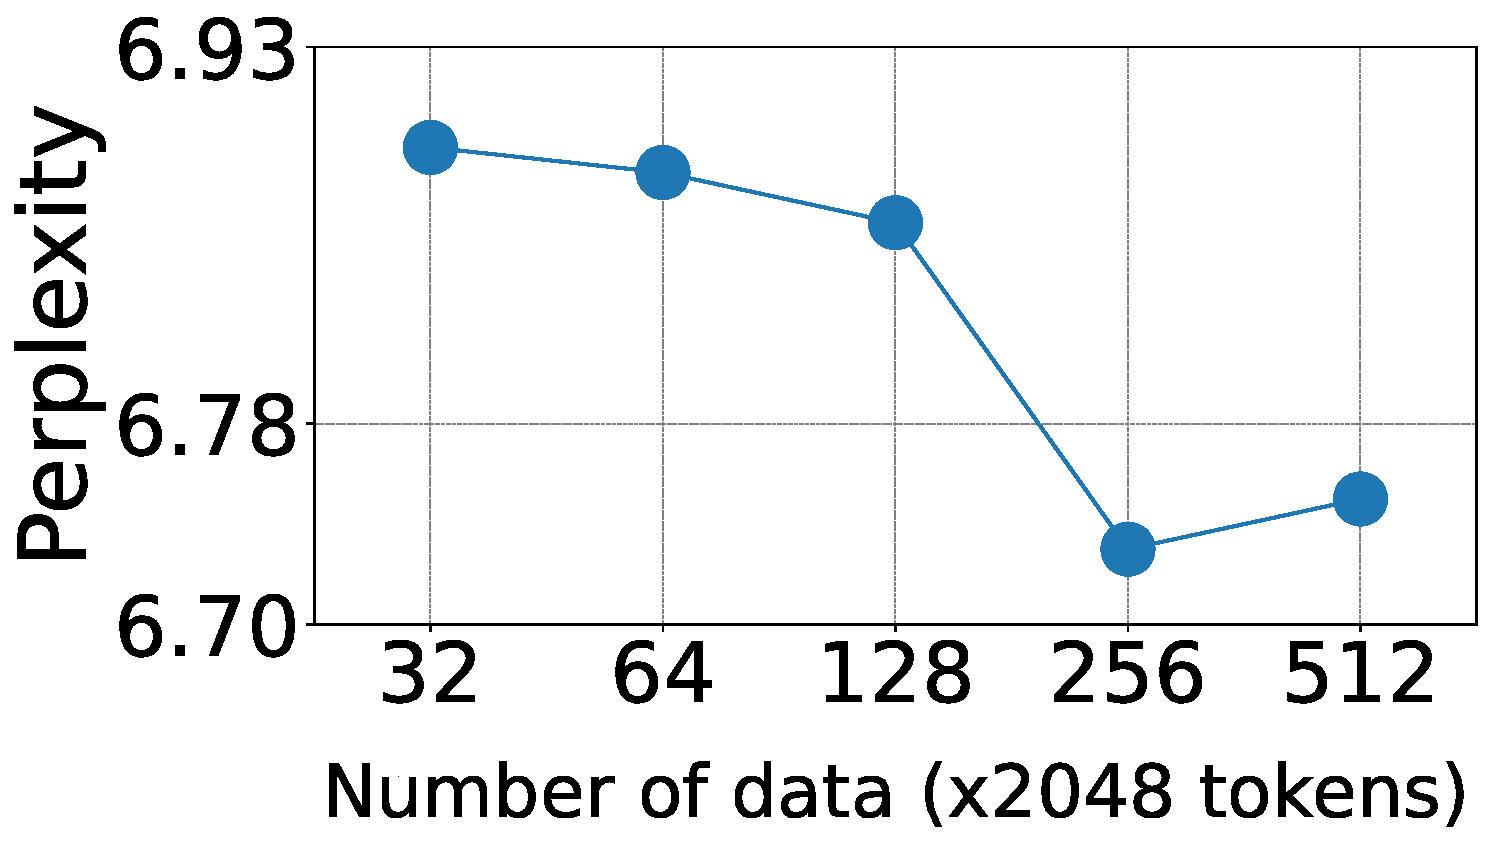
\includegraphics[width=0.455\textwidth]{Figures/cali_size.pdf}
        \label{fig:cali_size}
        }
        \subfigure[Change of Seed]{
        \centering
        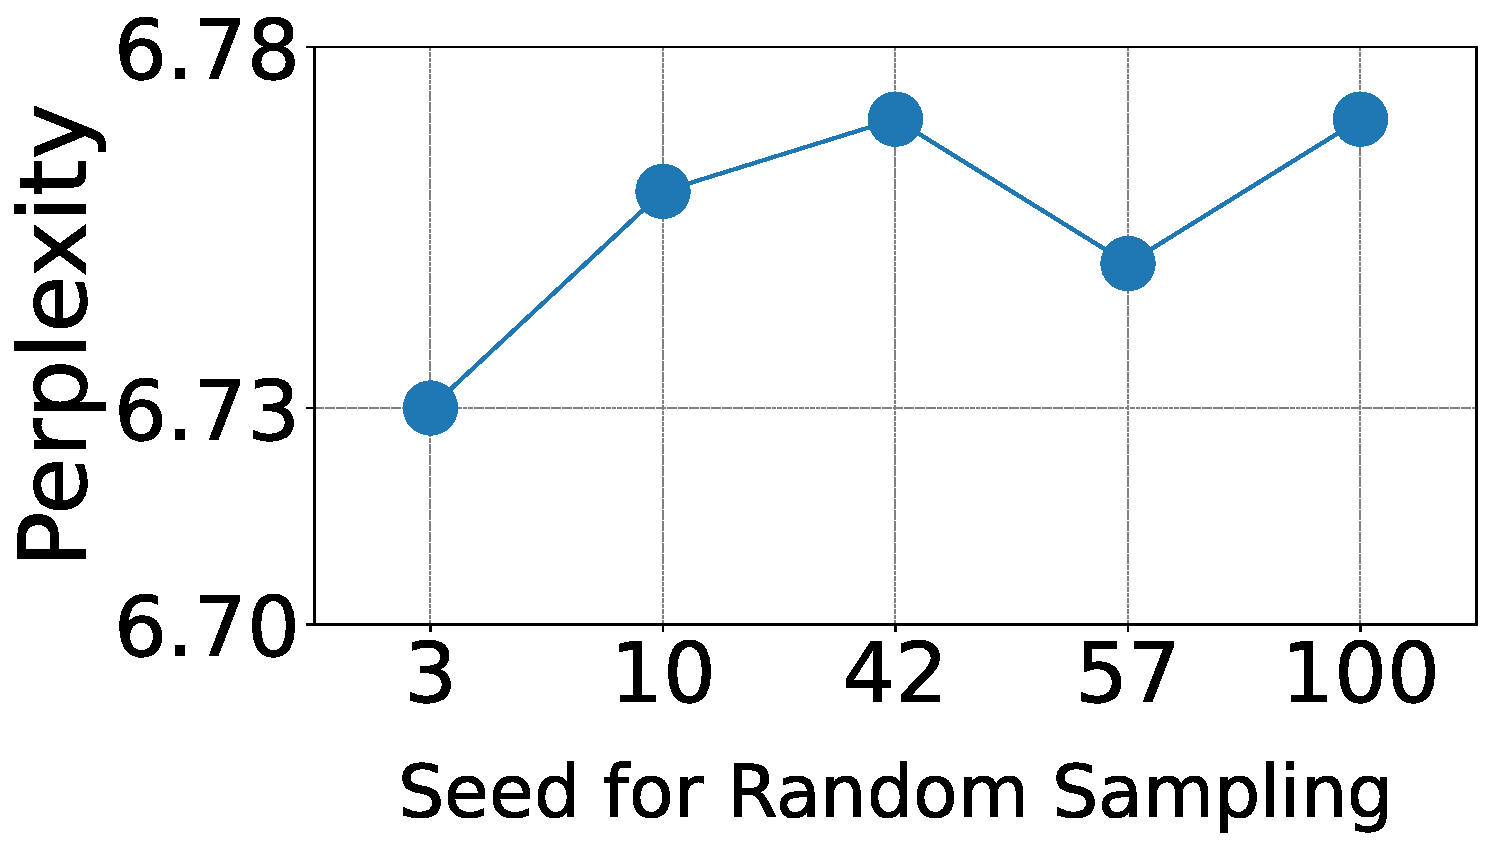
\includegraphics[width=0.45\textwidth]{Figures/seed.pdf}
        \label{fig:seed}
        }
        \vspace{-3mm}
        \DeclareGraphicsExtensions.
        \caption{Perplexity of LLaMA-7B under 20\% compression ratio using calibration data sampled with different number or  seeds from WikiText-2.}
        \label{fig:cali}
        \vspace{6mm}
        \loraTable
    \end{minipage}%
    \hspace{0.1cm}
    \begin{minipage}{0.485\textwidth}
    \vspace{3.5mm}
    \centering
    \datasetTable
\end{minipage}
\vspace{-3mm}
\end{figure}

\begin{figure}[t]
    \centering
    \begin{minipage}{.52\textwidth}
        \svdpruneTable
    \end{minipage}
    \hspace{0.1cm}
    \begin{minipage}{.45\textwidth}
      \svdquantTable
    \end{minipage}%
    % \vspace{-5mm}
\end{figure}


% \vspace{-2mm}
\subsection{Comparison with Other Types of LLM Compression Methods}
\label{subsection:Comparison_with_other_compression_methods}
\vspace{-1mm}
\sysname is orthogonal to other post-training LLM compression methods including pruning and quantization~\citep{DBLP:journals/tmlr/Wan0LA0LQYZZC024, shen2025efficient}. Lastly, we compare the performance of \sysname with state-of-the-art structured pruning-based and quantization-based LLM compression methods. As discussed in Section~\ref{sec:related_works}, since unstructured pruning methods are difficult to achieve its efficiency on hardware, we do not make a comparison with them in this experiment.

\vspace{-0mm}
\textbf{Comparison with Structured Pruning.}
First, we compare \sysname with three state-of-the-art structured pruning-based LLM compression methods: LLM-Pruner~\citep{DBLP:conf/nips/MaFW23}, SliceGPT~\citep{DBLP:conf/iclr/AshkboosCNHH24} and BlockPruner~\citep{DBLP:journals/corr/abs-2406-10594} under the same memory budget, ranging from 10 GB to 7 GB on LLaMA-7B using WikiText-2 dataset. 
%
As shown in Table~\ref{tab:svd_prune}, \sysname outperforms all three structured pruning-based LLM compression methods. In particular, \sysname achieves up to 56\% reduction in perplexity under 7G memory budget.

\vspace{-0mm}
\textbf{Comparison with Quantization.} Finally, we compare \sysname with three state-of-the-art quantization-based LLM compression methods: BiLLM~\citep{DBLP:conf/icml/HuangLQLZ0M024}, PB-LLM~\citep{DBLP:conf/iclr/YuanSD24}, and OneBit~\citep{DBLP:conf/nips/Xu0YWZLLC24}, which push the frontier to 1-bit quantization. 
%
Among them, both BiLLM and PB-LLM are post-training methods, and OneBit is training-required. 
%
The results on LLaMA-7B using WikiText-2 dataset are shown in Table~\ref{tab:svd_quant}. 
%
We have three observations. 
%
(1) Compared to post-training methods PB-LLM and BiLLM, \sysname achieves the best performance. 
%
(2) Training-required method OneBit outperforms \sysname. This result is expected because OneBit involves resource-intensive retraining using large-scale datasets to boost the accuracy after compression. %However, compared to post-training methods such as \sysname which does not require retraining, training-required method is way too expensive.
%
(3) Lastly, we combine \sysname with a 2-bit quantization-based post-training LLM compression method QuIP\#~\citep{DBLP:conf/icml/TsengCSKS24}. This is achieved by first applying \sysname to the LLM under 40\% compression ratio, and then applying QuIP\# for 2-bit quantization on the compressed model ($W'_u$ and $W'_v$) generated from \sysname. As shown in Table~\ref{tab:svd_quant}, \sysname outperforms state-of-the-art 1-bit training-required method OneBit \textit{without} involving resource-intensive retraining. This result demonstrates the potential of a hybrid approach -- integrating SVD-based and quantization-based compression techniques -- to push the boundaries of post-training LLM compression.


%by combining \sysname with a 2-bit quantization-based post-training LLM compression method QuIP\#~\citep{DBLP:conf/icml/TsengCSKS24}\footnote{\xin{This is achieved by first applying SVD-LLM to the LLM under 40\% compression ratio, and then applying QuIP\# for 2-bit quantization on the compressed model generated from SVD-LLM..}}, \sysname outperforms state-of-the-art 1-bit training-required method OneBit without involving resource-intensive retraining,  demonstrating the potential of a hybrid approach—integrating SVD-based and quantization-based compression techniques—to push the boundaries of post-training LLM compression.
%

%This result is important, because it introduces a highly efficient post-training approach that outperforms state-of-the-art 1-bit training-required quantization-based LLM compression method without incurring expensive retraining.

\vspace{-2mm}
\section{Conclusion}
\vspace{-2mm}
\label{sec:conclusion}
In this work, we present \sysname, a SVD-based
post-training LLM compression method. 
%
\sysname proposes a truncation-aware data whitening technique to guide which singular values to be truncated with minimal compression loss. It also introduces a sequential low-rank approximation strategy to compensate for accuracy degradation caused by singular value truncation.
%
We evaluate \sysname on $10$ datasets and seven models from three LLM families at three scales. Our results demonstrate
% that \sysname consistently outperforms state-of-the-art SVD-based LLM compression methods. Moreover, we demonstrate the inference efficiency of \sysname on real-world hardware and its superiority over other types of LLM compression methods.
%as well as KV cache reduction. 
 the superiority of SVD-LLM over state-of-the-arts, especially at high model compression ratios.

\vspace{-2mm}
\section{Acknowledgement}
\vspace{-2mm}

This work is supported in part by NSF Award NeTS-2312675.

\bibliography{Reference}
\bibliographystyle{plainnat}

\appendix
%%%%%%%%%%%%%%%%%%%%%%%%%%%%%%%%%%%%%%%%%%%%%%%%%%%%%%%%%%%%%%%%%%%%%%%%%%%%%%%
%%%%%%%%%%%%%%%%%%%%%%%%%%%%%%%%%%%%%%%%%%%%%%%%%%%%%%%%%%%%%%%%%%%%%%%%%%%%%%%
% APPENDIX
%%%%%%%%%%%%%%%%%%%%%%%%%%%%%%%%%%%%%%%%%%%%%%%%%%%%%%%%%%%%%%%%%%%%%%%%%%%%%%%
%%%%%%%%%%%%%%%%%%%%%%%%%%%%%%%%%%%%%%%%%%%%%%%%%%%%%%%%%%%%%%%%%%%%%%%%%%%%%%%
\newpage
\appendix
\onecolumn
\section{Appendix.}
\subsection{Pseudocode of \sysname}
\label{appendix:pseudocode}
\cref{algo:framework} shows the pseudocode of \sysname. Before compression, \sysname randomly collects a small amount of sentences as calibration data $C$, then runs the truncation-aware data whitening process as shown in~\cref{algo:whitening} to obtain the set of whitening matrix $\text{Set}_S$ for the weight to compress. After that, it runs the SVD and truncation with $\text{Set}_S$ on each weight matrix in the LLM. Instead of directly finishing the whole compression, it stores the decomposed matrices and further utilizes these matrices to run the parameter update with sequential low-rank approximation as shown in~\cref{algo:updating}.

\begin{algorithm}[ht]
\caption{Pseudocode of \sysname}
\begin{algorithmic}[1] % The number [1] tells LaTeX to number each line
\State \textbf{Input:} $M$: Original LLM
\State \textbf{Output:} $M''$: Compressed LLM by \sysname
\Procedure{\sysname}{$M$} % Algorithm name and parameters
    \State Randomly collect several sentences as the calibration data $C$
    \State $\text{Set}_S \gets \textproc{Truncation-Aware Data Whitening}(M, C)$
    \State $\text{Set}_W \gets M$ \Comment{Obtain the set of weights in $M$ to compress} 
    \For{$W$ \textbf{in} $\text{Set}_W$}
        \State $S \gets \text{Set}_S(W)$  \Comment{Extract the whitening matrix of current weight $W$} 
        \State $U, \Sigma, V \gets \operatorname{SVD}(WS)$   \Comment{Apply singular value decomposition on $W$}
        \State $\Sigma_1 \gets \operatorname{Trunc.}(\Sigma)$  \Comment{Truncate the smallest singular values in $\Sigma$}
        \State $W'_u \gets U(\Sigma_1)^{1/2}, W'_v \gets (\Sigma_1)^{1/2}V^TS^{-1}$ \Comment{Obtain two low-rank matrices}
        \State $M'(W) \gets W'_u, W'_v$      \Comment{Replace $W$ with $W'_u$ and $W'_v$ in $L$}
    \EndFor
    \State $M'' \gets \textproc{Parameter Update with Sequential Low-rank Approximation}(M')$
     \State \Return{$M''$}
\EndProcedure
\end{algorithmic}
\label{algo:framework}
\end{algorithm}

\begin{algorithm}[ht]
\caption{Pseudocode of Truncation-Aware Data Whitening}
\begin{algorithmic}[1] % The number [1] tells LaTeX to number each line
\State \textbf{Input:} $M$: Original LLM
\State \textbf{Input:} $C$: Calibration Data
\State \textbf{Output:} $\text{Set}_S$: Set of whitening matrices for the weight to compress in $M$
\Procedure{Truncation-Aware Data Whitening}{$M,C$} % Algorithm name and parameters
    \State $\text{Set}_S \gets \emptyset$  \Comment{Initialize the set of whitening matrices} 
    \State $\text{Set}_W \gets M$ \Comment{Obtain the set of weights in $M$ to compress} 
    \For{$W$ \textbf{in} $\text{Set}_W$}
        \State $X \gets M(W, C)$ \Comment{Obtain the input activation of the weight matrix $W$}
        \State $S \gets \operatorname{Cholesky\_Decomposition}(XX^T)$  \Comment{Apply cholesky decomposition on $XX^T$ }
        \State $\text{Set}_S \gets S \cup \text{Set}_S$  \Comment{Store the whitening weight matrix in the set}
    \EndFor
     \State \Return{$\text{Set}_S$}
\EndProcedure
\end{algorithmic}
\label{algo:whitening}
\end{algorithm}

\begin{algorithm}[ht]
\caption{\xin{Pseudocode of Parameter Update with Sequential Low-rank Approximation}}
\begin{algorithmic}[1] % The number [1] tells LaTeX to number each line
\State \textbf{Input:} $M'$: Compressed LLM by Truncation-aware Data Whitening
\State \textbf{Output:} $M''$: Compressed LLM with Parameter Update with Sequential Low-rank Approximation
\Procedure{Parameter Update with Sequential Low-rank Approximation}{$M'$} % Algorithm name and parameters
    \State $M'_u \gets \operatorname{LoRA_u}(M')$  \Comment{Fix all $W'_v$, fine-tune all $W'_u$}
    \State $M'' \gets \operatorname{LoRA_v}(M'_u)$  \Comment{Fix all $W'_u$, fine-tune all $W'_v$}
      \State \Return{$M''$}
\EndProcedure
\end{algorithmic}
\label{algo:updating}
\end{algorithm}


\subsection{Compression Loss of ASVD}
\label{subsec:ASVD_reconstruction_error}
%
ASVD introduces a diagonal scaling matrix $S_0$ that modifies the weight matrix to reflect the varying significance of different input channels. The linear layer is formulated as $Y=(WS_0)S_0^{-1}X$. The compression is made by keeping the largest $m$ singular value of $WS_0$:

\begin{align*}
WS_0 \approx & \sum_{i=1}^m \sigma'_i u'_i {v'}_i^T
\end{align*}
The resulting activation is expressed as:
\begin{align*}
    Y \approx & \sum_{i=1}^m \sigma'_i u'_i {v'}_i^T S_0^{-1}X ~.
\end{align*} 

The compression error $L=||(WS_0-\sum_{i=1}^{m}\sigma'_i u'_i {v'}_i^T)S_0^{-1}X||_F$ is demonstrated below:

\begin{align*}
L^2 =& ||(WS_0-\sum_{i=1}^{m}\sigma'_i u'_i {v'}_i^T)S_0^{-1}X||_F^2 \\
=& \left|\left|\sum_{i=m+1}^r \sigma'_iu'_i{v'}_i^{T}S_0^{-1}X\right|\right|_F^2 \\
=& \sum_{j=m+1}^r\sum_{i=m+1}^r \sigma'_i\sigma'_j\boldsymbol{\operatorname{Trace}}(u'_i {v'}_i^T X X^T v'_j {u'}_j^T) \\
=& \sum_{j=m+1}^r\sum_{i=m+1}^r \sigma'_i\sigma'_j\boldsymbol{\operatorname{Trace}}({u'}_j^T u'_i {v'}_i^T S_0^{-1}X X^T (S_0^{-1})^Tv'_j) \\
%=& \sum_{i=m+1}^r\sigma_i^2~trace(u_i v_i^T X X^T v_i u_i^T) + \\
%& \underset{i \neq j}{\sum_{j=m+1}^r\sum_{i=m+1}^r} \sigma_i\sigma_j~trace(u_i v_i^T X X^T v_j u_j^T) \\
=& \sum_{i=m+1}^r{\sigma'}_i^2\boldsymbol{\operatorname{Trace}}({v'}_i^T S_0^{-1}X X^T (S_0^{-1})^T v'_i) \\
=& \sum_{i=m+1}^r{\sigma'}_i^2~||{v'}_i^T S_0^{-1} X||_F^2 ~,
\end{align*}

which is still a complex function that involves the activation $X$, the diagonal matrix $S_0$, the singular vector $v'_i$ and the singular value $\sigma'_i$. As a result, compression error is not directly related to the singular value, and the conventional SVD compression by truncating the smallest singular values may lead to suboptimal compression error.

%You can have as much text here as you want. The main body must be at most $8$ pages long.
%For the final version, one more page can be added.
%If you want, you can use an appendix like this one.  

%The $\mathtt{\backslash onecolumn}$ command above can be kept in place if you prefer a one-column appendix, or can be removed if you prefer a two-column appendix.  Apart from this possible change, the style (font size, spacing, margins, page numbering, etc.) should be kept the same as the main body.
%implementation, hyperparameter for lora, generated contents for compressed/uncompressed model,compression time-consuming
%%%%%%%%%%%%%%%%%%%%%%%%%%%%%%%%%%%%%%%%%%%%%%%%%%%%%%%%%%%%%%%%%%%%%%%%%%%%%%%
%%%%%%%%%%%%%%%%%%%%%%%%%%%%%%%%%%%%%%%%%%%%%%%%%%%%%%%%%%%%%%%%%%%%%%%%%%%%%%%

\subsection{Compression Loss of \sysname}
\label{appendix:compression_loss_svdllm}
In \sysname, we also formulate the linear layer as $Y=(W S) S^{-1} X$, where $S^{-1} X X^T\left(S^{-1}\right)^T=I$. The compression is made by keeping the largest $m$ out of total $r$ singular values of $W S$. The compression loss $L$ is demonstrated as:

\begin{align*}
L^2 &=\left\|W X-W^{\prime} X\right\|_F^2=\left\|W S S^{-1} X-\boldsymbol{\operatorname{SVD}}(W S) S^{-1} X\right\|_F^2\\
& =\left\|(W S-\boldsymbol{\operatorname{SVD}}(W S)) S^{-1} X\right\|_F^2 \\
& =\left\|\left(W S-\sum_{i=1}^m \sigma_i u_i v_i^T\right) S^{-1} X\right\|_F^2 \\
& =\left\|\sum_{i=m+1}^r \sigma_i u_i v_i^T S^{-1} X\right\|_F^2 \\
& =\sum_{j=m+1}^r \sum_{i=m+1}^r \sigma_i \sigma_j \boldsymbol{\operatorname{Trace}}\left(u_i v_i^T S^{-1} X X^T\left(S^{-1}\right)^T v_j u_j^T\right) \\
& =\sum_{j=m+1}^r \sum_{i=m+1}^r \sigma_i \sigma_j \boldsymbol{\operatorname{Trace}}\left(u_i v_i^T\left(S^{-1} X X^T\left(S^{-1}\right)^T\right) v_j u_j^T\right) \\
& =\sum_{j=m+1}^r \sum_{i=m+1}^r \sigma_i \sigma_j \boldsymbol{\operatorname{Trace}}\left(u_i v_i^T v_j u_j^T\right) \\
\end{align*}
$$\because v_i^T v_i=u_i^T u_i=1 ; v_i^T v_j=u_i^T u_j=0, \boldsymbol{\operatorname{Trace}}\left(v_i v_i^T\right)=\boldsymbol{\operatorname{Trace}}\left(u_i u_i^T\right)=1, \forall i \neq j $$

$$\therefore L^2=\sum_{j=m+1}^r \sum_{i=m+1}^r \sigma_i \sigma_j \boldsymbol{\operatorname{Trace}}\left(u_i v_i^T v_j u_j^T\right)\\
=\sum_{i=m+1}^r \sigma_i^2 \boldsymbol{\operatorname{Trace}}\left(u_i v_i^T v_i u_i^T\right)=\sum_{i=m+1}^r \sigma_i^2$$

Therefore, the squared loss $L^2$ is equal to the sum of the squared singular values. Therefore, truncating the smallest singular values achieves the lowest compression loss.


\begin{figure}[t]
    \centering
    \subfigure[$W_Q\times S_Q$]{
        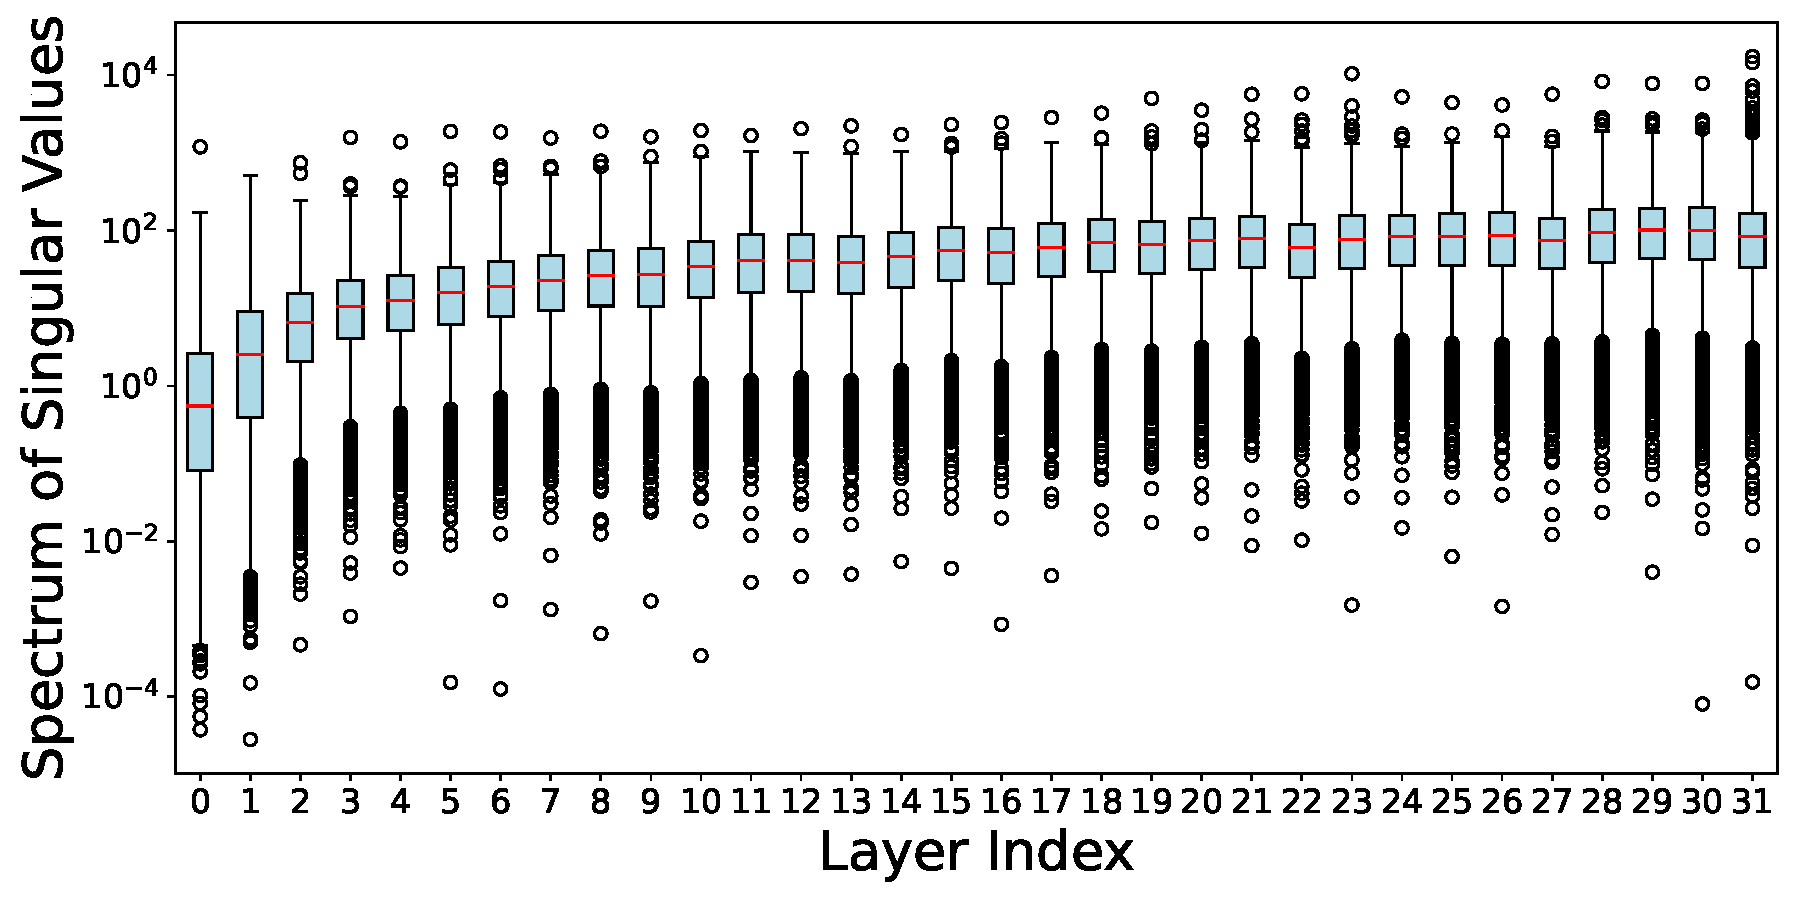
\includegraphics[width=1\textwidth]{Figures/q.pdf}
        \label{fig:q_spectrum}
    }
    \\
    \centering
    \subfigure[$W_K\times S_K$]{
        \includegraphics[width=1\textwidth]{Figures/K.pdf}
        \label{fig:v_spectrum}
    }
    \DeclareGraphicsExtensions.
    \caption{The singular value spectrum of the decomposed matrices across layers in LLaMA-7B.}
    \label{fig:spectrum_analysis}
\end{figure}

%\subsection{Implementation Details}
%\textbf{Implementation Details.} 
%\label{appendix:experimental_setup}
%To ensure a fair comparison, we followed ASVD~\citep{DBLP:journals/corr/abs-2312-05821} to randomly select 256 samples from WikiText-2 as the calibration data. 
%We followed the same configuration used in LLM-Pruner~\citep{DBLP:conf/nips/MaFW23} to use Alpaca~\citep{alpaca} dataset with 50K samples for parameter update in \sysname.
% All of our experiments are conducted on NVIDIA A100 GPUs.
%The inference efficiency experiment is conducted on both NVIDIA A100 GPU and AMD EPYC 7643 CPU while the other experiments are conducted on NVIDIA A100 GPUs.

\subsection{Spectrum Analysis of Singular Values decomposed by \sysname}
\label{appendix:spectrum_analysis}
In general, SVD is useful for compression when the matrix to be compressed shows a sharp decay of the singular values. Since \sysname decomposes the multiplication of the weight matrix $W$ and its corresponding whitening matrix $S$ instead of the original weight matrix $W$, which is different from the weight decomposition in the previous work~\citep{DBLP:journals/corr/abs-2312-05821,DBLP:conf/iclr/HsuHCLSJ22}, to study whether SVD compression is also applicable in \sysname, we select the Query ($W_Q$) and Key ($W_K$) weight matrices and show the spectrum of singular values of their multiplication with corresponding whitening matrices $S_Q$ and $S_K$. As shown in Figure~\ref{fig:spectrum_analysis}, most of the single values are less than or around 100 with only a few extremely large values, indicating that SVD is applicable in \sysname.


\subsection{Comparison with DRONE}
\label{appendix:comparison_with_drone}
\xin{
Previous work DRONE~\citep{DBLP:conf/nips/ChenYDH21} also proposes their data-aware method for SVD compression. They even provide a theoretical analysis to prove the optimal solution that their method achieves. Specifically, DRONE represents the low-rank compressed weight matrix $W'$ by $WM$. It performs SVD on both weight matrix $W = U_wS_wV_w^{T}$ and the transpose of input activation $X^T = U_xS_xV_x^{T}$ and then split these decomposed matrices as follows:}

$$
\begin{aligned}
& U_W=\left[\begin{array}{ll}
U_{W, r} & \bar{U}_{W, r}
\end{array}\right], S_W=\left[\begin{array}{cc}
S_{W, r} & 0 \\
0 & 0
\end{array}\right], V_W=\left[\begin{array}{ll}
V_{W, r} & \bar{V}_{W, r}
\end{array}\right] \\
& U_X=\left[\begin{array}{ll}
U_{X, t} & \bar{U}_{X, t}
\end{array}\right], S_X=\left[\begin{array}{cc}
S_{X, t} & 0 \\
0 & 0
\end{array}\right], V_X=\left[\begin{array}{ll}
V_{X, t} & \bar{V}_{X, t}
\end{array}\right] .
\end{aligned}
$$
\xin{
where $r$ and $k$ are the rank of the $W$ and $X$. $U_{W, r}, V_{W, r}, U_{X, t}, V_{X, t}$ denote corresponding row spaces and column spaces and $\bar{U}_{W, r}, \bar{V}_{W, r}, \bar{U}_{X, t}, \bar{V}_{X, t}$ are null spaces. Through theoretical deduction, DRONE converts the minimization of compression loss $||WX-W'X||_F = ||WX-WMX||_F$ to the minimization of $\left\|S_{W, r} V_{W, r}^T V_{X, t} S_{X, t}-S_{W, r} V_{W, r}^T M V_{X, t} S_{X, t}\right\|_F$, whose optimal value $L_{min}$ is the rank-k truncated SVD of $Z=S_{W, r} V_{W, r}^T V_{X, t} S_{X, t}$ by the fundamental property of SVD decomposition. To achieve the optimal value, DRONE formulates a solution $M = V_{W, r} S_{W, r}^{-1} Z_k S_{X, t}^{-1} V_{X, t}^T$, where $Z_k$ is the rank-k SVD truncation of $Z$. }

\xin{In short, compared with DRONE, \sysname is also optimal with the same theoretical compression loss as DRONE. Moreover, \sysname has \textbf{three} key advantages. Below is our detailed explanation.}


\xin{\textbf{\sysname is also optimal with the same theoretical compression loss as DRONE.}
% Although the motivation of \sysname originates from the SVD-based LLM compression methods, especially ASVD, and its motivation is to align the SVD truncation with the truncated singular values for a correct truncation, as discussed in Section 3.1, our theoretical analysis shows that \sysname is also optimal with the same compression loss as DRONE. 
The theoretical minimum compression loss $L_{min}$ is the F-norm loss of rank-k SVD truncation of $WX$, which has also been achieved by DRONE in their paper. Unlike DRONE, \sysname constructs the whitening matrix $S$ so that $S^{-1}X$ is orthonormal. Therefore, we have $||AS^{-1}X||_F = ||A||_F$. Suppose that we decompose $S$ with SVD to $U_s,S_s,V_s$, we can have $S_s = S_x$, $U_s = U_x, Us = Ux, V_s = QV_x$, where $Q$ is an orthogonal matrix. The matrix $WS$ to which \sysname applies SVD could be represented by $U_wS_wV_w^{T}U_sS_sV_s^{T}$. Suppose that we use $\boldsymbol{\operatorname{Trunc.}}(C)$ to represent the rank-k truncation of the matrix $C$ during SVD compression, the compression loss $L$ is derived as follows:}


\vspace{-5mm}
{\small
\begin{align*}
L &= ||WX-W'X||_F = ||(WSS^{-1}X -\boldsymbol{\operatorname{SVD}}(WS)S^{-1}X)||_F  = ||(WS -SVD(WS))S^{-1}X||_F\\
& = ||\boldsymbol{\operatorname{Trunc.}}(WS)S^{-1}X||_F = ||\boldsymbol{\operatorname{Trunc.}}(WS)||_F\\
&=||\boldsymbol{\operatorname{Trunc.}}(U_wS_wV_w^{T}U_sS_sV_s^{T})||_F =||\boldsymbol{\operatorname{Trunc.}}(WXQ^T)||_F = L_{min}
\end{align*}
}


\xin{Therefore, \sysname shares the same theoretical compression loss as DRONE. }



\xin{\textbf{Advantage \#1: DRONE incurs out-of-memory when compressing LLMs due to its requirement of storing the full large-scale activations, whereas \sysname is feasible.} To achieve data-awareness during compression, DRONE caches all input activations $X$ and spans them to calculate the corresponding singular vectors and singular values. In the DRONE paper, the authors apply DRONE to small LMs such as BERT. However, the activations generated by LLMs are often extremely large and are much larger than BERT. 
For example, to compress LLaMA-7B with 5,000 calibration data by DRONE, the total memory to cache the activation for a single weight matrix at a time is 5000 (data number) $\times$ 256 (seq\_len) $\times$ 11008 (dim) $\times$ 32 (fp32) $\div$ 1024 $\div$ 1024 $\div$ 1024 $=$ 419GB, which is more than 5 times larger than the memory provided by the NVIDIA A100 GPU, which has 80GB memory. Therefore, applying DRONE for LLM compression is infeasbile.  }

% \begin{wrapfigure}{r}{0.7\textwidth} % "r" 表示右侧，"0.5\textwidth" 控制宽度
%   \centering
%   \vspace{-5mm}
%   \dronelossTable
%   \vspace{-2mm}
% \end{wrapfigure}
\dronelossTable

\xin{In contrast, \sysname incrementally updates its $XX^T$ matrix by adding the $xx^T$ of each new input $x$. As such, \sysname eliminates the need to store the full activations, which requires only the storage of the matrix $XX^T$, which is considerably smaller than the full input activation. To compress LLaMA-7B with 5,000 calibration data, \sysname requires only 11008 $\times$ 11008 $\times$ 32 $\div$ 1024 $\div$ 1024 $\div$ 1024 $=$ 3.6GB. Compared to DRONE, \sysname achieves 116.38 times less memory reduction than DRONE. In our paper, we use WikiText-2 as a dataset. If we use DRONE, the total memory to cache the activation of a single weight matrix is larger than 24,600GB. In contrast, \sysname still requires 3.6GB of memory, which is more than 6,000 times less than DRONE. Due to this advantage, \sysname is much more practical to compress LLMs of size 7B or larger compared to DRONE.}

 \dronetimeTable
% \begin{wrapfigure}{r}{0.7\textwidth} % "r" 表示右侧，"0.5\textwidth" 控制宽度
%   \centering
%   \vspace{-5mm}
%   \dronetimeTable
% \end{wrapfigure}
\xin{\textbf{Advantage \#2: \sysname incurs much shorter compression time compared to DRONE.} DRONE involves more complex matrix operations, leading to longer compression time compared to \sysname. To illustrate this, we measured the time required by DRONE and \sysname to compress randomly generated weight and activation matrices of varying shapes under 50\% compression ratio. The results show that \sysname is approximately three times faster than DRONE.}

\xin{\textbf{Advantage \#3: \sysname has better numerical stability, which leads to superior empirical compression loss.}
 While \sysname shares the same theoretical compression loss as DRONE, DRONE’s higher complexity—stemming from additional SVD operations and inverse calculations on large-scale matrices—makes it less numerically stable compared to \sysname. This often results in higher empirical compression losses. To illustrate this, we compare \sysname and DRONE in terms of empirical compression losses for randomly generated matrices of various shapes. We also include the theoretical minimum value, represented by the rank-k Frobenius norm loss of $WX$. The results are summarized in the following table. As shown, we observe that \sysname achieves lower empirical compression losses than DRONE, underscoring its superior numerical stability.}



\flapTable

\subsection{Comparison with FLAP}
\label{appendix:flap_comparison}
\xin{
Recent work FLAP~\citep{DBLP:conf/aaai/AnZYTW24} is also a post-training structured-pruning method. Below we compare the perplexity of \sysname and FLAP on WikiText-2 under different compression ratios when compressing LLaMA-7B. As shown in~\cref{tab:flap}, \sysname consistently outperforms FLAP, especially under high compression ratios. }


\scalingTable

\subsection{Comparison with smaller LLMs pre-trained from scratch}
\label{appendix:pretrained_comparison}
To compare the performance between \sysname and scratch training, following the previous experimental design~\citep{DBLP:conf/nips/MaFW23}, we compress LLaMA-7B to the size of the 3B parameter with \sysname and select StableLM-3B~\citep{StableLM-3B-4E1T} as the baseline for comparison. As shown in Table~\ref{tab:scaling}. LLaMA-3B compressed from LLaMA-7B by \sysname achieves better accuracy in all datasets, indicating that \sysname could even achieve better accuracy than some scratch training methods. Furthermore, \sysname ensures higher throughput and lower memory consumption than StableLM-3B as shown in the table, which also meets our efficiency analysis and discussion in Section~\ref{subsec:inference_speedup}. 
% In the future, even though more and more smaller but more powerful LLMs will be obtained via scratch training, \sysname still holds its superiority from two aspects: (1) compressing more advanced larger LLMs to a smaller size with better accuracy. (2) Ensuring better inference efficiency with larger speedup and memory saving.


% \begin{wrapfigure}{r}{0.7\textwidth} % "r" 表示右侧，"0.5\textwidth" 控制宽度
%   \centering
%   \vspace{-5mm}
%   \timeTable
% \end{wrapfigure}

\timeTable

\subsection{Compression Speed Evaluation}
\label{appendix:compression_speed}
% \vspace{-2mm}
In addition to compression performance, we also evaluate the compression speed of \sysname and the baselines. Specifically, we measured the GPU hours used for \sysname and ASVD when compressing LLaMA-7B under 20\% compression ratio on an A100 GPU. The results are shown in~\cref{tab:time}. As shown, ASVD takes about $5.5$ hours, while \sysname completes the compression process in $3.5$ hours, which is $36\%$ times faster. When breaking down the time, most of the time consumed by ASVD is dedicated to searching for the specific compression ratio for each weight matrix based on its calculated importance score. In contrast, \sysname maintains a consistent compression ratio in all weight matrices and thus eliminates the time-consuming search process.

\subsection{Contents Generated from LLMs Compressed by \sysname and ASVD}
\label{sec:appendix_example}
Some examples of sentences generated by LLaMA-7B compressed with \sysname and ASVD are shown in~\cref{tab:visualization_lora}. 
%
The sentences generated by the model compressed by \sysname exhibit better fluency, relevance, and informativeness compared to those compressed by ASVD. More importantly, when the compression ratio is increased to 40\%, the previous state-of-the-art method ASVD completely loses its generation ability. 
In contrast, even when the compression ratio is up to 80\%, \sysname is still capable of generating complete sentences.
\exampleLoraTable




% \vspace{-3mm}


% \subsection{Comparison on extremely large-scale and more recent LLMs}
% \begin{wrapfigure}{r}{0.4\textwidth} % "r" 表示右侧，"0.5\textwidth" 控制宽度
%   \centering
%   \vspace{-4mm}
%   \morellmaccuracyTable
% \end{wrapfigure}

% \xin{
% To further show the generalization of \sysname, we compare its performance with other SVD-based baselines on extremely large-scale and more recent LLMs. Below shows the perplexity of \sysname and other baselines on WikiText-2 when compressing LLaMA-2 70B~\citep{DBLP:journals/corr/abs-2307-09288} and LLaMA-3 8B~\citep{DBLP:journals/corr/abs-2407-21783} under 20\% compression ratio. For LLaMA-2 70B, we only apply truncation-aware data whitening of \sysname without parameter update with sequential low-rank approximation due to the limited computational budget. OOM means that running the algorithm causes out-of-memory on 4 A100 GPUs. As shown, \sysname still consistently outperforms other baselines when applied on these two LLMs.}





\subsection{More Ablation Studies}
\label{appendix:more_ablation}
\xin{
\textbf{\sysname + Normal LoRA Fine-tuning v.s. \sysname + Sequential LoRA fine-tuning.} To illustrate the superiority of the designed parameter update with the sequential low-rank approximation in \sysname, which is a kind of sequential LoRA fine-tuning strategy over the normal LoRA fine-tuning strategy, we compare the compression performance of \sysname by applying either of these two fine-tuning strategies. Let's denote \sysname (SFT) as \sysname by applying sequential LoRA fine-tuning and \sysname (NFT) as \sysname by applying normal LoRA fine-tuning. As shown in~\cref{tab:lora_add}, \sysname (SFT) consistently outperforms \sysname (NFT), which also reaffirms our analysis in~\cref{subsec:lora_finetunig} that optimizing both low-rank matrices $W_u, W_v$ at the same time is not stable and may lead to poor fine-tuning performance.}

\loraaddTable

\xin{
\textbf{ASVD + Sequential LoRA Fine-tuning v.s. \sysname + Sequential LoRA Fine-tuning.} Although the designed sequential LoRA fine-tuning strategy could also be applied in other SVD-based LLM compression methods, other methods' performance is still poorer than \sysname even when integrated with this strategy for enhancement. To illustrate this, we compare the performance of the previous state-of-the-art method ASVD when applied with the sequential LoRA finetuning with \sysname. Let's denote \sysname (SFT) as \sysname by applying sequential LoRA fine-tuning and ASVD (SFT) as ASVD by applying sequential LoRA fine-tuning. As shown in~\cref{tab:lora_add}, \sysname (SFT) consistently outperforms ASVD (SFT) under various compression ratios.}

% \begin{wrapfigure}{r}{0.4\textwidth} % "r" 表示右侧，"0.5\textwidth" 控制宽度
%   \centering
%   \vspace{-3mm}
%   \orthoTable
% \end{wrapfigure}
% \xin{
% \textbf{Orthogonality of whitening matrix on inference activations.} 
% Below we randomly select three weight matrices $W_1,W_2,W_3$ in LLaMA-7B and compute their on-the-fly whitening matrix $S_{fly}$ computed during inference. To test whether $S_{pre}$ precomputed on the calibration data can also make the inference activation orthogonal like $S_{fly}$, we measure the difference between $S_{fly}S_{fly}^T$ and $S_{pre}S_{pre}^T$ in the MSE format, e.i., $\frac{1}{N}||S _{fly} S _{fly}^T-S _{pre} S _{pre}^T||_F^2$, where $N$ is the number of elements in $S _{pre}S _{pre}^T$. As shown in~\cref{tab:orthogonality}, the difference is small, indicating that the pre-computed whitening matrix $S _{pre}$ is still effective in making the inference activation orthogonal to ensure the alignment between SVD truncation and compression loss.}

\subsection{Limitations}
There are three limitations of \sysname, which are left for future work.

\textbf{(1) The compression accuracy still needs to be improved under the high compression ratio.}
Although \sysname has achieved the state-of-the-art performance compared to previous works such as FWSVD and ASVD, its compression accuracy still suffers from degradation, especially under the high compression ratio. To enhance the practicability of \sysname in real-world scenario, its accuracy should be at least comparable to that of the quantization method, including both low-bit and high-bit quantization, rather than being combined with the quantization methods for usage.

\textbf{(2) The latency of \sysname needs to be optimized while being used to compress the KV cache.} As discussed in~\cref{subsec:inference_speedup}, \sysname can also be applied to compress the KV cache for memory saving during inference. However, this benefit does not come free. In fact, due to the additional calculation caused by recovering the original key and value states, the inference speed will be impacted by compressing the KV cache with \sysname, which should be optimized in the future.


\textbf{(3) \sysname should be better guided for high-quality generation.} Although \sysname achieves low perplexity, as demonstrated in~\cref{tab:dataset_acc}, it is still possible to generate low-quality content, such as repeated words even under low compression ratios. This phenomenon of compressed LLM has also been mentioned in previous work~\citep{DBLP:conf/nips/MaFW23} and should be eliminated in the future by guiding the compressed LLM for outputting high-quality generation.


\end{document}